\documentclass[11pt,a4paper]{article}

\usepackage[margin=1in, paperwidth=8.3in, paperheight=11.7in]{geometry}
\usepackage{amsfonts}
\usepackage{amsmath}
\usepackage{amssymb}
\usepackage{dsfont}
\usepackage{enumerate}
\usepackage{enumitem}
\usepackage{fancyhdr}
\usepackage{graphicx}
\usepackage{tikz}
\usepackage{changepage} 

\begin{document}

\pagestyle{fancy}
\setlength\parindent{0pt}
\allowdisplaybreaks

\renewcommand{\headrulewidth}{0pt}

\hyphenpenalty 10000
\exhyphenpenalty 10000

% Cover page title
\title{Machine Learning - Reviewed Notes}
\author{Dom Hutchinson}
\date{\today}
\maketitle

% Header
\fancyhead[L]{Dom Hutchinson}
\fancyhead[C]{Machine Learning - Reviewed Notes}
\fancyhead[R]{\today}

% Default enumerate labeling
\setlist[enumerate,1]{label={\roman*)}}

% Counters
\newcounter{definition}[section]
\newcounter{example}[section]
\newcounter{notation}[section]
\newcounter{proposition}[section]
\newcounter{proof}[section]
\newcounter{remark}[section]
\newcounter{theorem}[section]

% commands
\newcommand{\dotprod}[0]{\boldsymbol{\cdot}}
\newcommand{\cosech}[0]{\mathrm{cosech}\ }
\newcommand{\cosec}[0]{\mathrm{cosec}\ }
\newcommand{\sech}[0]{\mathrm{sech}\ }
\newcommand{\prob}[0]{\mathbb{P}}
\newcommand{\nats}[0]{\mathbb{N}}
\newcommand{\cov}[0]{\mathrm{Cov}}
\newcommand{\var}[0]{\mathrm{Var}}
\newcommand{\expect}[0]{\mathbb{E}}
\newcommand{\reals}[0]{\mathbb{R}}
\newcommand{\integers}[0]{\mathbb{Z}}
\newcommand{\indicator}[0]{\mathds{1}}
\newcommand{\nb}[0]{\textit{N.B.} }
\newcommand{\ie}[0]{\textit{i.e.} }
\newcommand{\eg}[0]{\textit{e.g.} }
\newcommand{\X}[0]{\textbf{X}}
\newcommand{\x}[0]{\textbf{x}}
\newcommand{\iid}[0]{\overset{\text{iid}}{\sim}}
\newcommand{\proved}[0]{$\hfill\square$\\}

\newcommand{\definition}[1]{\stepcounter{definition} \textbf{Definition \arabic{section}.\arabic{definition}\ - }\textit{#1}\\}
\newcommand{\definitionn}[1]{\stepcounter{definition} \textbf{Definition \arabic{section}.\arabic{definition}\ - }\textit{#1}}
\newcommand{\proof}[1]{\stepcounter{proof} \textbf{Proof \arabic{section}.\arabic{proof}\ - }\textit{#1}\\}
\newcommand{\prooff}[1]{\stepcounter{proof} \textbf{Proof \arabic{section}.\arabic{proof}\ - }\textit{#1}}
\newcommand{\example}[1]{\stepcounter{example} \textbf{Example \arabic{section}.\arabic{example}\ - }\textit{#1}\\}
\newcommand{\examplee}[1]{\stepcounter{example} \textbf{Example \arabic{section}.\arabic{example}\ - }\textit{#1}}
\newcommand{\notation}[1]{\stepcounter{notation} \textbf{Notation \arabic{section}.\arabic{notation}\ - }\textit{#1}\\}
\newcommand{\notationn}[1]{\stepcounter{notation} \textbf{Notation \arabic{section}.\arabic{notation}\ - }\textit{#1}}
\newcommand{\proposition}[1]{\stepcounter{proposition} \textbf{Proposition \arabic{section}.\arabic{proposition}\ - }\textit{#1}\\}
\newcommand{\propositionn}[1]{\stepcounter{proposition} \textbf{Proposition \arabic{section}.\arabic{proposition}\ - }\textit{#1}}
\newcommand{\remark}[1]{\stepcounter{remark} \textbf{Remark \arabic{section}.\arabic{remark}\ - }\textit{#1}\\}
\newcommand{\remarkk}[1]{\stepcounter{remark} \textbf{Remark \arabic{section}.\arabic{remark}\ - }\textit{#1}}
\newcommand{\theorem}[1]{\stepcounter{theorem} \textbf{Theorem \arabic{section}.\arabic{theorem}\ - }\textit{#1}\\}
\newcommand{\theoremm}[1]{\stepcounter{theorem} \textbf{Theorem \arabic{section}.\arabic{theorem}\ - }\textit{#1}}

\tableofcontents

% Start of content
\newpage

\section{General}

\remark{Machine Learning}
\textit{Machine Learning} is a class of techniques which use algorithms \& statistical models with the goal of producing systems which can perform a specific task without being given explicit instructions for how to do so. \textit{Machine Learning} problems can be broken down into three sub-problems
\begin{enumerate}
	\item How can we formulate beliefs \& assumptions about a scenario mathematically?
	\item How can we connect our assumptions with observed data?
	\item How can we update our beliefs using the observed data?
\end{enumerate}

\definition{Reasoning}
Reasoning is the process of applying premises which are known to be true to infer whether an unseen statement is true. 
\begin{enumerate}
	\item \textit{Deductive Reasoning} assumes that the premises supply \underline{all} the information required to make a definite conclusion about the truefullness of the unseen statement.\\
	\eg When it rains things outside get wet. Grass is outside therefore when it rains outside grass gets wet.
	\item \textit{Inductive Reasoning} assumes that the premises supply \underline{some} of the information and thus does \underline{not} produce a definite conclusion.\\
	\eg The grass has gott wet when it rains, numerous times, therefore when it rains grass gets wet.
	\item \textit{Abductive Reasoning} takes a conclusion \& a rule and tries to infer the premises for them.\\
	\eg The grass is wet. Grass gets wet when it rains, therefore it has rained outside.
\end{enumerate}

\definition{Bayesian Inference}
\textit{Bayesian Inference} is a method of inference in which \textit{Bayes' Theorem} is used to update a \textit{posterior} distribution as more information about the \textit{prior} \& \textit{likelihood} is discovered.\\

\definition{Intractable}
A problem is said to be \textit{Intractable} if there is no known algorithm for solving it. There are two common reasons for a problem to be \textit{Intractable}
\begin{enumerate}
	\item \textit{Computationally Intractable} - A given formulation is impossible to solve (typically due to an integration).
	\item \textit{Analytically Intractable} - Due to some limitation in observation techniques we are not able to fully define a scenario.
\end{enumerate}

\remarkk{Free-Lunch Theorem}
\begin{quotation}
\textit{There are an infinite number of hypotheses that perfectly explain all the observed data. Adding a data point removes an infinite number of these possibilities, but still leaves an infinite number.}
\end{quotation}

\remark{Models do not need ot be perfectly true to be useful.}

\definition{Training Data}
Let $\X\in\reals^{D\times N}$ represent $N$ $D$-dimensional sets of independent variables and $\textbf{y}\in\reals^N$ be the outcomes (dependent variables) for each of these sets.\\
\textit{Training Data} is the pair $(\X,\textbf{y})$ which we use to learn the relationship between the domain and output space of a scenario.\\
\nb \textit{Test Data} has the same structure as \textit{Training Data} except we apply our learned process to the parameters and then compare our learned outcomes to the true outcomes in order to assess our model.\\

\definition{Model}
A \textit{Model} is a system that models relationships between several variables. Generally this is occurs when consider independent \& dependent variables.\\
Models are built upon two types of variables
\begin{enumerate}
	\item \textit{Observable Variables} - A variable whoses value can be observed directly.
	\item \textit{Latent Variables} - A variable that cannot be directly observed, but a model is dependent upon it, thus we must infer their values from \textit{Observable Variables}.
\end{enumerate}

\definition{Discriminative Model}
Let $X$ be a set of observed values.\\
A \textit{Discriminative Model} aims to find the distribution for the outcomes, $Y$ produced by $X$.
$$p(Y|X)$$
\eg $k$-Nearest Neighbours, Neural Networks, Logistic Regression.\\

\definition{Generative Model}
Let $Y$ be a set of observed outcomes.\\
A \textit{Generative Model} aims to find a distribution for the variables, $X$, which produced $Y$.
$$p(X|Y)$$
\eg Gaussian Mixture Model, Latent Dirichlet Allocation, everything else discussed here.\\

\definition{Mixture Model}
\textit{Mixture Models} represent the presence of subpopulations within an overall population, without requiring the training data to specify which subpopulation each data point belongs to.\\
Sometimes it makes sense to interpret these subpopulations as clusters (\eg$k$-means clustering), or as discrete latent variables which assign data points to specific subpopulations (\eg Gaussian Mixtures Model).

\subsection{Supervised Learning}

\definition{Supervised Learning}
Let $(\X,\textbf{y})$ be \textit{Training Data}.\\
\textit{Supervised Learning} is the process of learing a function, $f(\cdot)$, which maps the domain space to the output space.
$$y_i=f(\x_i)$$
\nb Often we assume that there is some \textit{Additive Noise}, $y_i=f(\x_i)+\varepsilon$ with $\varepsilon\sim\text{Normal}(0,1)$.

\subsubsection{Neural Network}

\definition{Neural Network}
\textit{Neural Networks} are a system that aims to learn how to perform a task without the rules being defined explicitly. A \textit{Neural Network} is built layers of \textit{neurons} where each neuron has a uni-directional edge to every node in the next layer. Each \textit{neuron} assigns a weight to the edges entering it \& has a threshold function which determines whether it fires.\\

\proposition{Neural Network Layers}
The layers of a \textit{Neural Network} are split into three categories
\begin{itemize}
	\item[-] \textit{Input Layer} - We use inputted data to decide which of these \textit{neurons} fires. There is one \textit{neuron} for each possibility in the input space (\eg one per pixel in an image).
	\item[-] \textit{Hidden Layers} - These lie between the \textit{input} \& \textit{output layers} and do not necessarily have the same number of \textit{neurons}. Each \textit{neuron} a function which defined how much signal it sends to the next layer, dependent upon the signals it recieves.
	\item[-] \textit{Output Layer} - Has one \textit{neuron} for each possible output class. The class of the \textit{neuron} with the greatest value is returned as the result of the computation.
\end{itemize}

\proposition{Functions for Hidden Layer}
The function assigned to each \textit{neurons} in the hidden layer should be defined st if they get enough stimuli from its connected \textit{neurons} then it sends a signal to the next layer.\\
A common way to do this is to calculate
$$t:=w_0+\sum_{i=1}^nw_iz_i$$
where $w_0$ is a bias, $w_i$ is the weight assigned to the $i^\text{th}$ edge \& $z_i$ is the signal recived from the $i^\text{th}$ edge, and then to pass a linear transformation of this through the \textit{sigmoid} function.\\

\proposition{Training a Neural Network}
To train a \textit{Neural Network} we typically define an \textit{Error Function}, $E(\textbf{w})$, which assesses how good our classifier is for a given set of weights. We then seek the set of weights, $\hat{\textbf{w}}$, which minimises the \textit{Error Function}.\\
A popular \textit{Error Function} is the \textit{Sum-of-Squares Error} function
$$\hat{\textbf{w}}:=\text{argmin}_\textbf{w}E(\textbf{w})\text{ where }E(\textbf{w}):=\frac12\sum_{i=1}^N\|y(\x_i,\textbf{w})-\textbf{t}_i\|^2$$
where $\{(\x_i,\textbf{t}_i)\}$ is our \textit{training data} and $y(\cdot)$ is the output our neural network gives.\\
\nb \textit{Gradient Descent} is a popular minimisation technique.\\

\remark{In many cases the error function is independent for each training item ${E(\cdot)=\sum_{n=1}^NE_n(\cdot)}$}

\proposition{Backpropogation}
Let $E(\cdot)$ be an \textit{Error Function} used to evaluate our \textit{Neural Network}.\\
\textit{Backpropogation} is a technique for training a \textit{Neural Network} and is based on evaluating the gradient of the \textit{Error Function}, $\nabla E(\cdot)$.\\
Consider the simple case were
$$y_k(\x,\textbf{w}):=\sum_iw_{ki}x_i\text{ and }E_n(\textbf{w}):=\frac{1}{2}\sum_k(y_k(\x_n,\textbf{w})-t_{nk})^2$$
The gradient of the error function wrt a specific weight, $w_{ji}$, is
$$\frac{\partial E_n}{\partial w_{ji}}=(y_j(\x_n,\textbf{w})-t_{nj})x_{ni}$$
This can be calculated for every edge \& then the weight applied to each edge can be updated accordingly by adding/subtracting a certain amount of this gradient to its weight.

\subsection{Un-Supervised Learning}

\definition{Un-Supervised Learning}
\textit{Unsupervised Learning} is the set of \textit{Machine Learning} algoirthms which seek to make inferences from unlabeled data. Our task is to take a set of observations, $\textbf{Y}$ and infer a \textit{Latent Representation} for the model, $\X$, \& a function, $f$, that maps from the \textit{Latent Space} to the \textit{Observed Space}.\\
\nb Techinically defining $f(x)=x$ would suffice so we need to add some supervision (direction) to produce a meaningful result.\\

\remark{Latent Space, $\X$}
Since we are seeking the \textit{Latent Sapce} we can make assumptions about its distribtion. Typically this is that each variable is centred around 0, is independent of all others \& has variance $1$.
$$\X\sim\text{Normal}(\textbf{0},I)$$

\remark{Preference}
In \textit{Unsupervised Learning} we often talk about \textit{Preference} rather than \textit{belief}. The idea being that if we get two equally good solutions we choose the one that we belive is more likely, \ie give greater preference to more likely solutions.\\
\nb \textit{Preference} is analoguous to \textit{Priors}.

\subsubsection{Principle Component Analysis}

\definition{Principle Component Analysis}
\textit{Principle Component Analysis} is an \textit{unsupervised learning} technique which projects observations into the $D$ dimensional plane which causes the greatest spread in the data.\\
Let $\textbf{Y}\in\reals^{N\times D}$ be a set of observed data and $\textbf{X}\in\reals^{N\times k}$ be the latent representation we wish to find
\begin{enumerate}
	\item Calculate the co-variance matrix for \textbf{Y}.
	\item Calculate the eigenvalues \& vectors for the covaraince matrix.
	\item Pick the $k$ largest eigenvalues \& use their corresponding eigenvectors as rows of $\textbf{W}\in\reals^{D\times k}$.
	\item Calculate $\X$ st $\textbf{Y}=\textbf{W}\X^T$.
\end{enumerate}

\proposition{Derivation of Principle Component Analysis}
Let $\textbf{Y}$ be a set of observations, $\X$ be the set of latent variables we wish to infer \& $\textbf{W}$ be a set of weightings which define a linear relationship between $\X$ \& $\textbf{Y}$.\\
We wish to derive a posterior distribution for $\textbf{W}$ \& $\X$, our unknown parameters.\\
We define a \textit{Likelihood Function}
$$p(\textbf{Y}|\textbf{W},\X)=\text{Normal}\left(\X\textbf{W}+\mu,\frac1\beta I\right)$$
where $\mu$ is a constant offest.\\
This leads to the following joint distribution
$$p(\textbf{Y},\textbf{W},\X)=p(\textbf{Y}|\textbf{W},\X)p(\X)p(\textbf{W})$$
We can now marginalise our $\X$ \& $\textbf{W}$
$$p(\textbf{Y})=\int p(\textbf{Y}|\textbf{W},\X)p(\X)p(\textbf{W})$$
This is intractable (\ie we cannot solve for both $\textbf{W}$ \& $\X$) so we must take a point estimate of one \& intergrate out the other.\\
Since we wish to be able to take unseen data \& infer its latent location we need to be able to calculate $p(\x|\textbf{y})$ and this can only be reached if we marginalise out $\X$ (\ie estimate $\textbf{W}$).\\
$$p(\X,\textbf{Y}|\textbf{W})=p(\textbf{Y}|\textbf{W},\X)p(\X)$$
We know both the left hand terms
\[\begin{array}{rcl}
p(\textbf{Y}|\textbf{W},\X)&=&\text{Normal}\left(\X\textbf{W}+\mu,\frac{1}{\beta}I\right)\\
p(\X)&=&\text{Normal}(\textbf{0},I)
\end{array}\]
Consider a pair of points $(\x,\textbf{y})$ then.
$$p(\textbf{y},\x|\textbf{W})=\text{Normal}\left(\begin{pmatrix}\expect(\textbf{y})\\\expect(\x)\end{pmatrix}\begin{pmatrix}\expect[(\textbf{y}-\expect(\textbf{y}))(\textbf{y}-\expect(\textbf{y}))^T]&\expect[(\textbf{y}-\expect(\textbf{y}))(\textbf{x}-\expect(\textbf{x}))^T]\\\expect[(\textbf{x}-\expect(\textbf{x}))(\textbf{y}-\expect(\textbf{y}))^T]&\expect[(\textbf{x}-\expect(\textbf{x}))(\textbf{x}-\expect(\textbf{x}))^T]\end{pmatrix}\right)$$
Note that
$$\expect(\textbf{y})=\expect[\textbf{W}\x+\mu+\varepsilon]=\textbf{W}\expect(\x)+\mu+\expect(\mu)=\textbf{W}\times0+\mu+0=\mu$$
Thus
\[\begin{array}{rcl}
\expect[(\textbf{x}-\expect(\textbf{x}))(\textbf{y}-\expect(\textbf{y}))^T]&=&\expect[\x(\textbf{y}-\mu)^T]\\
&=&\expect[\x(\textbf{W}\x+\mu+\varepsilon-\mu)^T]\\
&=&\expect[\x(\textbf{W}\x)^T+\x\varepsilon^T]\\
&=&\expect(\x\x^T\textbf{W}]+\expect(\x)\expect(\varepsilon)\\
&=&\expect(\x\x^T)\textbf{W}^T+0\\
&=&I\textbf{W}^T\\
&=&\textbf{W}^T\\
\implies\expect[(\textbf{y}-\expect(\textbf{y}))(\textbf{x}-\expect(\textbf{x}))^T]&=&\textbf{W}\\
\text{and }\expect[(\textbf{y}-\expect(\textbf{y}))(\textbf{y}-\expect(\textbf{y}))^T]&=&\expect[(\textbf{W}\x+\mu+\varepsilon-\mu)(\textbf{W}\x+\mu+\varepsilon-\mu)^T]\\
&=&\expect[\textbf{W}\x(\textbf{W}\x)^T+\textbf{W}\x\varepsilon+\varepsilon\textbf{W}\x^T+\varepsilon\varepsilon^T]\\
&=&\expect[\textbf{W}\x\x^T\textbf{W}]+\expect[\textbf{W}\x\varepsilon^T]+\expect[\varepsilon\x^T\textbf{W}^T]+\expect(\varepsilon\varepsilon^T)\\
&=&\textbf{W}I\textbf{W}^T+\textbf{W}\times0+0\times\textbf{W}^T+\sigma^2 I\\
&=&\textbf{W}\textbf{W}^T+\sigma^2I\\
\implies p(\textbf{y},\x|\textbf{W})&=&\text{Normal}\left(\begin{pmatrix}\mu\\\textbf{0}\end{pmatrix},\begin{pmatrix}\textbf{W}\textbf{W}^T+\sigma^2I&\textbf{W}\\\textbf{W}^T&I\end{pmatrix}\right)\\
\implies p(\textbf{y}|\textbf{W})&=&\text{Normal}(\mu,\textbf{W}\textbf{W}^T+\sigma^2I)\\
\text{and }p(\x|\textbf{y},\textbf{W})&=&\text{Normal}(\textbf{W}^T(\textbf{W}\textbf{W}^T+\sigma^2I)^{-1}(\textbf{y}-\mu),\ I-\textbf{W}^T(\textbf{W}\textbf{W}^T+\sigma^2I)^{-1}\textbf{W})\\
\end{array}\]
Now we need to make estimate \textbf{W}.\\
We can estimate the maximum likelihood solution for \textbf{W} by finding the eigenvalues \& vectors for the covariance function of the observed data, \textbf{Y}, and then using the eigenvectors with the $D$ largest associated eigenvalues as rows of \textbf{W}.\footnote{This works since we assume that precision tends to infty, $\beta\to\infty$}.\\
Where $D$ is the dimensionality we wish our result to have.

\subsection{Parametric Models}

\subsubsection{Topic Model}

\remark{Motivation}
\textit{Topic Models} are based on the premise that certain types of data can be well desribed by atomic units within them. (\ie A document can be well described by the words within it).\\

\definition{Topic Models}
\textit{Topic Models} are a class of models designed to discover the \textit{topics} which occur in a collection of documents. \textit{Latent Dirichlet Allocation} is a common topic model.\\

\remark{See \textbf{Proposition 2.6} for an implementation.}

\subsection{Non-Parametric Models}

\subsubsection{$k$-Nearest Neighbours}

\definition{$k$-Means Clustering}
\textit{$k$-Means Clustering} produces $k$ clusters by partitioning a set of $n$ observations. \textit{$k$-Means Clustering} assumes the covariance of each cluster is similar. \textit{$k$-Means Clustering} aims to find a configuration of clusters that minimise \textit{Within-Cluster Scatter}. A typical technique for \textit{$k$-Means Clustering} is
\begin{enumerate}[label=\arabic*)]
	\item Randomly initialise $k$ vectors, $\{\mu_1,\dots,\mu_k\}$.
	\item
	\begin{enumerate}
		\item Assign each training instance to its nearest $\mu_i$.
		\item Move each $\mu_i$ to be the centroid of the instances assigned to it.
	\end{enumerate}
	\item Repeat $2)$ until no $\{\mu_1,\dots,\mu_k\}$ moves.
\end{enumerate}
\nb This finds a local minimum, not necessarily a global minimum.\\

\definition{$k$-Medoids Clustering}
\textit{$k$-Medoids Clustering} is a variation on \textit{$k$-Means Clustering} where, instead of using any point as a centre, it uses training  observations as the centre of a cluster.

\subsubsection{Gaussian Mixture Models}

\definition{Mixture of Gaussians}
A \textit{Mixture of Gaussians} is a superposition of $K$ Gaussian distributions of the form
$$p(\x)=\sum_{k=1}^K\pi_k\text{Normal}(\x|\pmb\mu_k,\pmb\Sigma_k)\text{ where }\sum_{i=1}^K\pi_i=1$$
where each distribution has its own \textit{mean} \& \textit{co-variance} and is given a relative weighting, \textit{Mixing Coefficient}, $\pi_i$.\\
\nb Each distribution is referred to as a \textit{Component} of the mixture.\\

\proposition{Gaussian Mixture Models}
Let $\x$ be distributed according to a \textit{Mixture of Gaussians}.\\
Consider a binary $k$-dimensional random variable $\textbf{z}$ where all but one dimension is zero-valued and define the  marginal distribution $p(\textbf{z})$ st $p(z_i=1)=\pi_i$ (\nb This is the same \textit{Mixing Coefficient}).\\
Since $\textbf{z}$ is zero-valued in all bar one dimension
\[\begin{array}{rrcl}
&p(\textbf{z})&=&\displaystyle\prod_{i=1}^K\pi_i^{z_i}\\
&p(\x|\textbf{z})&=&\displaystyle\prod_{i=1}^K\text{Normal}(\x|\pmb\mu_i,\pmb\Sigma_i)^{z_i}\\
&p(\x,\textbf{z})&=&p(\x|\textbf{z})p(\textbf{z})\\
&&=&{\displaystyle\prod_{i=1}^K\pi_i^{z_i}}\text{Normal}(\x|\pmb\mu_i,\pmb\Sigma_i)^{z_i}
\end{array}\]
\nb $\textbf{z}$ represents the cluster that a data point belongs to.\\

\proposition{Fitting a Gaussian Mixtures Model}
Consider wishing to fit $K$ $D$-dimensional components where $\textbf{Y}_k\sim\text{Normal}(\pmb\mu_k,\Sigma_k)$ for data points $\{\x_1,\dots,\x_n\}$.\\
(In this case we the covariance matrices are diagonal).
\begin{enumerate}
	\item $\forall\ k\in[1,K]$ random initalise $\textbf{Y}_k$.
	\item $\forall\ i\in[1,n]$ associate $\x_i$ to component $k$ where $\prob(\pmb\mu=\pmb\mu_k,\Sigma=\Sigma_k|\x_i)$ is greatest.
	\item $\forall\ k\in[1,K],\ d\in[1,D]$ set ${\displaystyle\mu_{k,d}=\frac1{n_k}\sum_{c_i=k}x_{i,d}}$ and ${\displaystyle\Sigma_{k,dd}=\frac{1}{n_k}\sum_{c_i=k}(x_{i,d}-\mu_{k,d})^2}$.\\
	where $n_k$ is the number of data points assigned to component $k$.
	\item Repeat until convergence of $\textbf{Y}_1,\dots,\textbf{Y}_K$.
\end{enumerate}
\nb These are the sample mean \& covariance. $\pmb\mu\in\reals^{D},\ \Sigma\in\reals^{D\times D}$.

\section{Probability}

\subsection{General}

\definition{Frequentist Probabiltiy}
\textit{Frequentist Probabiltiy} is an interpretation of \textit{Probability} where \textit{Probability} refers to the limiting relative frequences of events. \textit{Probabilities} are objective properties of the world.
$$P(X=x)=\lim_{n\to\infty}\dfrac{k}{n}$$
where $k$ is the number of times an observation of $x$ occurs in $n$ samples.\\

\definition{Bayesian Probability}
\textit{Bayesian Probability} is an interpretation of \textit{Probability} where \textit{Probability} is a reasonable expectation given our beliefs of the system. We encode these beliefs using the different components of \textit{Bayes' Theorem}.\\

\remark{In this course we mainly deal with Bayesian Probability}

\definition{Random Variable}
A \textit{Random Variable} is a function which maps an event in the sample space to a value.\\ $X$ is a \textit{Random Variable} if it satisfies the signature
$$X:\Omega\to\reals$$

\definition{Probability Measure}
\textit{Probability Measures} are functions which maps sets of events in a probability space to a value in $[0,1]$. The returned value is a measure of how likely it is for a realisation of the random variable to fulfil the criteria placed upon it.
$$p(\cdot):\mathcal{F}\to[0,1]$$
and must fulfil the following criteria
\begin{enumerate}
	\item $\forall\ A_0,\dots,A_n\in\mathcal{F}\implies\left(\bigcup\limits_{i=0}^nA_i\right)\in\mathcal{F}$.
	\item $p(\Omega)=1$.
	\item $p\left(\bigcup\limits_{i=0}^n\right)=\sum\limits_{i=0}^np(A_i)$ for any $n$ disjoint $A_0,\dots,A_n$.
\end{enumerate}

\definition{Joint Probability Measure}
A \textit{Joint Probability Measure} is a \textit{Probabiltiy Measure} which is defined over multiple random variables and measures how likely it is that a realisation of the random variables fulfils \underline{all} the criteria placed upon them.
$$p(\cdot,\cdot):X\times Y\to[0,1]$$
$$p(X=x,Y=Y)\equiv p(X=x\text{ and }Y=y)$$

\definition{Marginal Probability Measure}
A \textit{Marginal Probability Measure} is a \textit{Probabiltiy Measure} for a proper subset of the random variables in a scenario.\\
Suppose we have a scenario which is modelled by random variables $X$ \& $Y$ then $p(X)$ is a \textit{Marginal Probabiltiy Measure}.\\
\textit{Marginalisation} is the process of reformulating the \textit{Mariginal Distribution} of a single random variable to incorporate other random variables in the scenario
$$p(X)=\int p(X,Y=y)dy\text{ or }p(X)=\sum_i p(X,Y=y_i)$$

\definition{Conditional Probability Distribution}
A \textit{Conditional Probability Distribution} is a \textit{Probability Distribution} which measures the likelihood of a realisation of a random variable fulfilling a criteria placed upon it \textbf{given} that the realisation has already fulfilled a criteria placed upon another random variable.
$$p(X=x|Y=Y)\equiv p(X=x\text{ given we know that }Y=y)$$
\nb If $X$ \& $Y$ are independent then $p(X=x|Y=y)=P(X=x)$.\\

\definition{Independence}
Let $X$ \& $Y$ be \textit{Random Variables} and $p(\cdot)$ be a \textit{Probabiltiy Distribution}.\\
$X$ \& $Y$ are said to be \textit{independent} of one another if
$$p(X=x,Y=y)=p(X=x).p(Y=y)$$

\definition{Expected Value}
Let $X$ be a random variable, $p(\cdot)$ be a probability distribution for $X$ and $f(\cdot):\reals\to\reals$.\\
The \textit{Expected Value} of a \textit{Probability Distribution} is the mean value $X$.\\
If $X$ is \underline{continuous} then
$$\expect(X):=\int_{-\infty}^\infty xp(x)dx\text{ and }\expect(f(X)):=\int_{-\infty}^\infty f(x)p(x)dx$$
If $X$ is \underline{discrete} then
$$\expect(X):=\sum_{x=-\infty}^\infty xp(x)\text{ and }\expect(f(X)):=\sum_{x=-\infty}^\infty f(x)p(x)$$

\theorem{Linear Transformations of Expected Value}
Let $X$ be a random variable and $a,b\in\reals$. Then
$$\expect(aX+b)=a\expect(X)+b$$

\definition{Variance}
Let $X$ be a random variable.\\
\textit{Variance} measures how far a set of random numbers are spread from their expected value.
$$\var(X):=\expect(X-\expect(X))^2=\expect(X^2)-[\expect(X)]^2$$
where $\sigma^2$ \& $\Sigma$ are measures of variance.\\

\theorem{Linear Transformations of Variance}
Let $X$ be a random variable and $a,b\in\reals$. Then
$$\var(aX+b)=a^2\var(X)$$

\definition{Precision}
\textit{Precision} is the reciprical of \textit{Variance}.\\
$$\lambda:=\frac{1}{\sigma^2}$$
$$\Lambda=\begin{pmatrix}\Lambda_{11}&\Lambda_{12}&\dots&\Lambda_{1D}\\\Lambda_{21}&\Lambda_{22}&\dots&\Lambda_{2D}\\\vdots&\vdots&\ddots&\vdots\\\Lambda_{D1}&\Lambda_{D2}&\dots&\Lambda_{DD}\end{pmatrix}:=\begin{pmatrix}\Sigma_{11}&\Sigma_{12}&\dots&\Sigma_{1D}\\\Sigma_{21}&\Sigma_{22}&\dots&\Sigma_{2D}\\\vdots&\vdots&\ddots&\vdots\\\Sigma_{D1}&\Sigma_{D2}&\dots&\Sigma_{DD}\end{pmatrix}^{-1}$$

\definition{Covariance}
Let $X$ \& $Y$ be random variables.\\
\textit{Covariance}  measures the joint variability of two random variables.\\
$$\cov(X,Y)=\expect[(X-\expect(X))(Y-\expect(Y))]=\expect(XY)-\expect(X)\expect(Y)$$
If $X$ \& $Y$ are independent then $\cov(X,Y)=0$.\\
\nb By definition of \textit{Covaraince} $\cov(X,X)=\var(X)$.\\

\definition{Conjugacy}
A \textit{Prior} is said to be \textit{Conjugate} if its distribution is in the same family of distributions as the distribution of the \textit{Posterior}, in a given scenario.\\
\nb Tables of \textit{Conjugate Pairs} exist online.\\

\remark{Why use Conjugate Priors?}
If we have a \textit{Conjugate Prior} then we can determine the distribution of the \textit{Posterior} by passing the parameters of the \textit{Prior} though pre-derived functions and thus avoid computing the \textit{Evidence}, which is often difficult.
$$\text{Posterior}\propto\text{Likelihood}\times\text{Prior}$$

\remark{Usefulness of Conjugacy}
It is useful to use conjugacy as it allows us to avoid computing the \textit{Evidence} (from Bayes' Rule) and simply multipling the prior \& likelihood and then normalising to find the posterior.\\
However, in many cases, this is not possible and we have to perform a full calculation to reach the posterior.

\subsection{Theorems}

\theorem{Basic Rules}
Let $X$ \& $Y$ be \textit{Random Variables} and $p(\cdot)$ be a \textit{Probabiltiy Distribution}.
\begin{center}\begin{tabular}{|l|l|}
\hline
Product Rule&$p(X=x,Y=Y)=p(Y=y|X=x)p(X=x)$\\
\hline
Sum Rule&$p(X=x)=\sum_jp(X=x,Y=y_j)$\\
\hline
\end{tabular}\end{center}

\theorem{Bayes' Theorem}
Let $X$ \& $Y$ be \textit{Random Variables} and $p(\cdot)$ be a \textit{Probabiltiy Distribution}.\\
\textit{Bayes' Theorem} states that
$$p(X=x|Y=y)=\frac{p(Y=y|X=x)p(X=x)}{p(Y=y)}$$

\remark{Components of Bayes' Theorem}
Let $X$ \& $Y$ be \textit{Random Varaibles} where $Y$ is observed data \& $X$ represents the parameters of a theorised model of $X$, then the components of \textit{Baye's Theorem} can each be considered to explain a different part of a model
$$\underbrace{p(X|Y)}_\text{Posterior}=\frac{\overbrace{p(Y|X)}^\text{Likelihood}\overbrace{p(X)}^\text{Prior}}{\underbrace{p(Y)}_\text{Evidence}}$$
\begin{center}\begin{tabular}{|l|l|}
\hline
\textbf{Component}&\textbf{Description}\\
\hline
\textit{Posterior}&Which parameters are most likely to produce the data we observed.\\
\hline
\textit{Likelihood}&How likely is the observed data given these parameters\\
&\nb $p(X|\theta)=L(\theta|X)$\\
\hline
\textit{Prior}&Our prior assumptions about the distribution of the parameters\\
\hline
\textit{Evidence}&How likely is the observed data across all models\\
&\nb This normalises the distribution of the posterior\\
\hline
\end{tabular}\end{center}
\nb The \textit{Evidence} is normally the most challenging component of this relationship to calculate.\\

\theorem{Central Limit Theorem}
Let $\{X_n\}_{n\in\nats}$ be a sequence of independent \& indetically distributed with $\expect(X_i)=\mu<\infty$ and $\var(X_i)=\sigma^2<\infty$. Then\\
$$\sqrt\frac{n}{\sigma^2}(Z_n-\mu)\to_\mathcal{D}Z\sim\text{Normal}(0,1)$$

\subsection{Likelihood}

\definition{Likelihood Function}
Let $\X\sim f_n(\cdot;\theta^*)$ for some $\theta^*\in\Theta$ and $\x$ be a realisation of $\X$.\\
\textit{Likelihood Function}s are the family of functions which measure the probability of observing $\x$ given a value of the parameter $\theta$.
$$L(\theta;\x)\propto f_n(\x;\theta)$$
\nb AKA \textit{Obsevered Likelihood Function}.\\

\definition{Log-Likelihood Function}
Let $L(\cdot)$ be a likelihood function.\\
The \textit{Log-Likelihoof Function} of $L(\cdot)$ is the natural log of $L(\cdot)$
$$\ell(\theta;\x):=\ln L(\theta;\x)+C=\ln f_n(\x;\theta)+C\text{ for }C\in\reals$$
We use the \textit{Log-Likelihood} since it removes exponentials and makes products into summations, making many problems more tractable.\\
\nb $\ell(\cdot)$ is increasing with $L(\cdot)$.\\

\definition{Maximum Likelihood Estimate}
Let $\X\sim f_n(\cdot;\theta^*)$ for some $\theta^*\in\Theta$ and $\hat\theta$ be an esimate of the value of $\theta^*$.\\
$\hat\theta$ is the \textit{Maximum Likelihood Estimate} of $\theta^*$ if
\[\begin{array}{rcl}
\hat\theta&=&\text{argmax}_{\theta\in\Theta}L(\theta;\x)\\
&=&\text{argmax}_{\theta\in\Theta}\ell(\theta;\x)
\end{array}\]
\nb The \textit{Maximum Likelihood Estimate} of $\theta$ is often denoted as $\hat\theta_\text{MLE}$.\\

\propositionn{Finding the Maximum Likelihood Estimate}
\begin{enumerate}
	\item Define a \textit{Likelihood Function}, $L(\theta;\x)$.
	\item Get the \textit{Log-Likelihood Function}, $\ell(\theta;\x):=\ln L(\theta;\x)$.
	\item Take the derivative wrt each parameter, $\frac{\partial}{\partial\theta}\ell(\theta;\x)$.
	\item Set each derivative to 0 and solve to find stationary points for the parameters.
	\item If a stationary point is a maximum then it is a \textit{Maximum Likelihood Estimate}
\end{enumerate}

\definition{Type II Maximum Likelihood}
In some cases we are only able to marginialise some of the variables in a problem.\\
\textit{Type II Maximum Likelihood} is the process of marginialising out \& intergrating over all the variables we can and then maximising the remaining.\\
\nb This is used in Gaussian Processses.

\subsection{Evidence}
\remark{Also known as the \textit{Marginal Likelihood}.}

\definition{Evidence}
The \textit{Evidence} is the probability distribution that is left when we have integrated out everything except for the data.\\
Let $Y$ be a set of observed data \& $\theta$ be the set of parameters for a model we are theorising. Then the evidence is
\[\begin{array}{rcl}
p(Y)&=&\displaystyle\int_\theta p(Y|\theta)p(\theta)d\theta\\
p(Y)&=&\displaystyle\sum_\theta p(Y|\theta)p(\theta)
\end{array}\]
\nb The likelihood for observing the data we have, given all possible hypotheses about $\theta$.\\

\proposition{Evidence of a Model}
Let $\mathcal{D}$ be the observable-space, $M$ be a theorised model \& $\theta$ be the parameters that $M$ depends upon. Then the \textit{Evidence} for $M$ in $\mathcal{D}$ is the distribution
$$p(\mathcal{D}|M)=\int_\theta p(\mathcal{D}|M,\theta)p(\theta)d\theta$$
This requires us to define the \textit{Prior}, $p(\theta|M)$. As we do not know much about the possible parameters, we allow for a large range of possible values of $\theta$. One possibility is a zero-meaned Gaussian with high variance.\\
$$p(\theta|M)=\text{Normal}(\textbf{0},\sigma^2I)\text{ for large }\sigma^2$$

\definition{Na\"ive Monte Carlo Approach}
Performing the integration defined in \textbf{Proposition 2.2} is generally tricky so we use the 
\textit{Na\"ive Monte Carlo Approach} to approximate $p(\mathcal{D}|M)$.\\
Consider making samples, $\{\theta_1,\dots,\theta_S\}$, from the prior of the parameters.
$$p(\mathcal{D}|M)\approx\frac{1}{S}\sum_{s=1}^Sp(\mathcal{D}|M,\theta_s)\text{ where }\theta_s\sim p(\theta|M)$$

\remark{Comparing Models}
Suppose we observe some data $Y$, we can evaluate the probability of observing this under our \textit{Evidence}. The greater this probability is the greater the probabilitiy that the model we have chosen is the \textit{right} one.\\
This provides a metric for comparing multiple models and suggests choosing the model with the greatest likelihood, under our evidence, is better.\\

\remark{Choosing Models}
Suppose we can sort the observable-space in order of increasing complexity \& can work out the evidence for each model, at each point in the observation-space. Then we should \underline{pick the simplest} \underline{model which is able to explain our data}.\\
Let $\mathcal{D}$ be the known observable-space, $\mathcal{D}_0$ be a reasonable point in the observation space where we may make our observations and $\mathcal{M}_1,\mathcal{M}_2\ \&\ \mathcal{M}_3$ be models which explain $\mathcal{D}$.
\begin{center}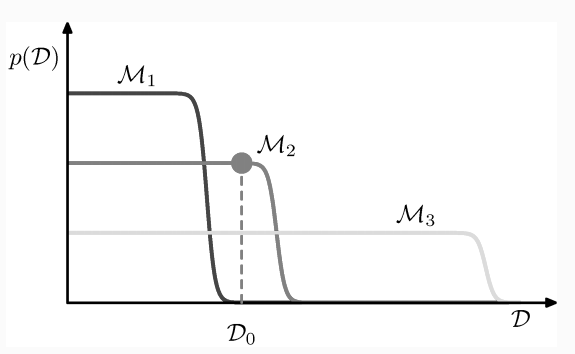
\includegraphics[scale=.5]{img/mackay.png}\end{center}
We see $\mathcal{M}_1$ is too simple to explain $\mathcal{D}_0$ \& $\mathcal{M}_3$ is unnecessarily complex (\ie explains too many factors). Thus we choose $\mathcal{M}_2$ in this case.\\
\nb This is an application of \textit{Occam's Razor}

\subsection{Stochastic Processes}

\definition{Stochastic Process}
A \textit{Stochastic Process} is a collection of random variables, all defined in the same probabilty space \& indexed by some set. Often the random variables are indexed by time or space.

\subsubsection{Gaussian Processes}

\definition{Gaussian Process}
Let $S$ be a set.\\
A \textit{Gaussian Process} on $S$ is a set of random variables $\{Z_t\}_{t\in S}$ such that $\forall\ n\in\nats,\ \forall\ t_1,\dots,t_n\in S$ the vector $\{Z_{t_1},\dots,Z_{t_n}\}$ is a \textit{Multivariate Gaussian}.\\
The distribution of a \textit{Gaussian Process} is the continuous joint distribution of the random variables which make it up.\\
For a \textit{Gaussian Process} we define functions for calculating the mean, $\mu(\cdot)$, \& covariance, $k(\cdot,\cdot)$. These functions only depend on the training data \& a few hard-coded parameters thus \textit{Gaussian Processes} are a \underline{non}-parametric.\\
\nb \textit{Covariance Functions} are \textit{Kernels}.\\

\remark{Verbose Definition of Gaussian Processes}
\textit{Gaussian Processes} are the family of \textit{Stochastic Processes} where each finite collection of the random variables has a \textit{Multivariate Normal Distribution}.\\

\remark{Gaussian Processes is the infinite dimensional generalisation of a Gaussian Distribution}

\remark{Sampling from a Gaussian Process}
When we sample a \textit{Gaussian Process} we are given a number of points from which we interpolate a function.\\

\proposition{Covariance Functions, $k(\cdot,\cdot)$}
Below are some common co-variance used for \textit{Gaussian Processess}
\begin{center}\begin{tabular}{|l|l|}
\hline
\textbf{Name}&\textbf{General Form}\\
\hline
Constant&$k(x,y)=c$\\
Linear&$k(x,y)=x^Ty$\\
White Gaussian Nose&$k(x,y)=\sigma^2\delta_{x,y}$\\
Squard Exponential&$k(x,y)=\sigma^2e^{-\frac{1}{2\ell^2}(x-y)^T(x-y)}$\\
Periodic&$k(x,y)=e^{-\frac2{\ell^2}\sin^2\left(\frac{1}{2}(x-y)\right)}$\\
\hline
\end{tabular}\end{center}
where $\sigma$ is a standard deviation parmater, $\ell$ is a length-scale parameter for the function \& $\delta_{x,y}$ is the \textit{Kronecker Delta}.\\

\proposition{Mean Function, $\mu(\cdot)$}
We typically assume that the \textit{Mean Function} is zero for all inputs as this simplifies a lot of calculations.
$$\mu(\x)=0\ \forall\ \x$$
To ensure this is a valid assumption we centre our data around 0 by subtracting the sample mean from each data point.
$$\x'=\x-\bar{\x}$$

\subsubsection{Dirichlet Processes}

\definition{Dirichlet Processes}
\textit{Dirichlet Processes} are the family of \textit{Stochastic Processes} whose realisations are probability distributions over a set $S$.\\
The \textit{Dirichlet Process} is a prior over countable infinite sets and used to generate a partitioning of a, possibly, infinite number of data points (Clusters).
\textit{Dirichlet Processes} are hard to define explicitly \& here shall be defined constructively.\\
\nb \textit{Dirichlet Processes} are distributions over distributions over a set $S$.\\

\remark{Dirichlet Processes Parameters}
\textit{Dirichlet Processes} are parameterised by a \textit{base distribution}, $f(\cdot)$, ${\text{and a \textit{concentration parameter}}, \alpha}$.\\

\remark{Dirichlet Processes are the infinite dimensional generalisation of a Dirichlet Distribution}

\remark{Application of Dirichlet Processes}
\textit{Dirichlet Processes} are used in scenarios where we do not know how many clusters our data has \& we do not wish to hard code a specific number for this. \textit{Dirichlet Processes} are able to grow the number of clusters as it recieves more data.\\

\proposition{Formulation of Dirichlet Processes - Chinese Restaurant Process}
Consider having an infinite number of tables (clusters) \& dishes (labels for clusters) and a finite number of customers (data points).\\
We allow any number of customers to sit at a table, but only ever allow one dish per table.\\
\textit{We consider how to distribute customers between tables.}\\
When a new customer arrives, the probability that they start a new table is
$$\frac\alpha{N+\alpha-1}$$
where $\alpha$ is a senstivity parameter that we set \& $N$ is the number of customers already in the restaurant.\\
If the customer chooses to not start a new table then they sit at table $i$ with probabiltiy
$$\frac{n_i}N$$
where $n_i$ is the number of customers already at table $i$ \& $N$ is the number of customers already in the restaurant.\\
By varying $\alpha$ we can perform simulations to determine how any tables are used \& how many people sit at each one.\\
Joining a new table is applied as sampling from the given distribution $f(\cdot)$ and joining an exisiting table is applied as sampling the value which formed the table.\\

\proposition{Formulation of Dirichlet Processes - Stick Breaking}
Consider taking a sample $\{x_1,x_2\dots\}$ from $\text{Beta}(1,\alpha)$ ($x_i\in[0,1]\ \forall\ i$).\\
Imagine having a stick. Each of these sampled values tells you what proporition of the remaining stick to break off.\\
Thus after $n$ samples $C_n:=x_n\prod_{i=1}^{n-1}x_i$ of the stick remains. Each portion can be considered a cluster.\\
Take a sample $\{z_1,z_2,\dots\}$ from the given distribution $f(\cdot)$.\\
Merge the sample to form a new distribution $g(z)=\sum_{k\in\nats}C_k\delta_{z_k,z}$.\\

\definition{Latent Dirichlet Allocation}
\textit{Latent Dirichlet Allocation}, LDA, is a \textit{Generative Model} used in natural language processing to find topics within a document. To do so, it makes the following assumptions
\begin{enumerate}
	\item Documents contain a variety of topics.
	\item For each topic their is a distribution of words which characterises it.
	\item The order of words is irrelevant.
\end{enumerate}
\nb Based on the premise that certain data types can be well explained by atomic units with them.\\

\propositionn{LDA Process}
\begin{enumerate}[label=\arabic*)]
	\item Assign each word in each document to a random topic.
	\item For each document, $d$
	\begin{enumerate}
		\item For each word, $w$, with current topic assignment $t$.
		\begin{enumerate}
			\item Assume all topic assignments are correct, except for the word currently being considered.
			\item Calculate two propotions
			\begin{itemize}
				\item[-] Proporition of words in $d$ that are currentlty assign to $t$. $$p(\text{Topic}=t|\text{Document}=d)$$
				\item[-] Proportion of occurences of $w$ (across all documents) \text{which are assigned to $t$.} $$p(\text{Word}=w|\text{Topic}=t)$$
			\end{itemize}
			\item Multiply the two proportions and assign $w$ to a new topic based on the resulting probability.
			$$p(\text{Topic}=t|\text{Document}=d)\times p(\text{Word}=w|\text{Topic}=t)$$
		\end{enumerate}
	\end{enumerate}
	\item Repeat until convergence.
\end{enumerate}

\proposition{Latent Dirichlet Allocation - Topic Model}
Let $\{\beta_1,\dots,\beta_T\}$ be the characteristic distribution of words for each possible topic and $w_{d,i}$ be the $i^\text{th}$ word in the $d^\text{th}$ document.\\
We want to find a distribution for the topics in each document, $\theta_d$.\\
Define $z_{d,i}$ to be the topic we assign to the $i^\text{th}$ word in the $d^\text{th}$ document.\\
We have the following dependencies
$$p(w_{d,i}|\pmb\beta,z_{d,i})\quad p(z_{d,i}|\theta_d)$$
Since we assume each word is independent we have a distribution for all words in a document
$$p(\textbf{w}_d|\pmb\beta,\textbf{z}_d)=\prod_{i=1}^Np(w_{d,i}|\pmb\beta,z_{d,i})$$
We assume that the distribution of topics in documents is independent \& the characteristic distribution for each topic is independent
$$p(\pmb\theta)=\prod_{i=1}^Dp(\theta_d)\text{ and }p(\pmb\theta)=\prod_{i=1}^Tp(\beta_i)$$
Given a final joint distribution
$$p(w,z,\pmb\theta,\pmb\beta)=\underbrace{\prod_{t=1}^Tp(\beta_t)\underbrace{\prod_{d=1}^Dp(\theta_d)\underbrace{\prod_{i=1}^Np(w_{d,i}|\pmb\beta,z_{d,i})p(z_{d,i}|\theta_d)}_\text{word}}_\text{document}}_\text{corpus}$$
We still have to choose the form of each distribution. A good set of choices is
\[\begin{array}{rcl}
\beta_k&\sim&\text{Dirichlet}(\eta)\\
\theta_d&\sim&\text{Dirichlet}(\alpha)\\
z_{d,i}&\sim&\text{Multi-Normal}(\theta_d)\\
w_{d,i}&\sim&\text{Multi-Normal}(\beta_{z_{d,i}})\\
\end{array}\]
where $\eta\ \&\ \alpha$ are sensitivity parameters that we set

\subsection{Distributions}

\definition{$\beta$-Distribution}
Let $X\sim\text{Beta}(\alpha,\beta)$.\\
A \textit{continuous} random variable with shape parameters $\alpha,\beta>0$. Then
\[\begin{array}{rcl}
f_X(x)&\propto&x^{\alpha-1}(1-x)^{\beta-1}\mathds{1}\{x\in[0,1]\}\\
\expect(X)&=&\dfrac{\alpha}{\alpha+\beta}\\
\var(X)&=&\dfrac{\alpha\beta}{(\alpha+\beta)^2(\alpha+\beta+1)}\\
\mathcal{M}_X(t)&=&1+{\displaystyle\sum_{k=1}^\infty\left(\prod_{r=0}^{k-1}\dfrac{\alpha+r}{\alpha+\beta+r}\right)\dfrac{t^k}{k!}}
\end{array}\]
\nb Beta-Distributions are used to encode our prior beliefs about the distribution of the parameters.\\

\definition{Bernoulli Distribution}
Let $X\sim\text{Bernoulli}(p)$.\\
A \textit{discrete} random variable which takes 1 with probability $p$ \& 0 with probability $(1-p)$. Then
\[\begin{array}{rcl}
p_X(k)&=&\begin{cases}1-p&\text{if }k=0\\p&\text{if }k=1\\0&\text{otherwise}\end{cases}\\
P_X(k)&=&\begin{cases}0&\text{if }k<0\\1-p&\text{if }k\in[0,1)\\1&\text{otherwise}\end{cases}\\
\expect(X)&=&p\\
\var(X)&=&p(1-p)\\
\mathcal{M}_X(t)&=&(1-p)+pe^t
\end{array}\]
\nb Often we define $q:=1-p$ for simplicity.\\

\definition{Binomial Distribution}
Let $X\sim\text{Binomial}(n,p)$.\\
A \textit{discrete} random variable modelled by a \textit{Binomial Distribution} on $n$ independent events and rate of success $p$.
\[\begin{array}{rcl}
p_X(k)&=&{n\choose k}p^k(1-p)^{n-k}\\
P_X(k)&=&\sum_{i=1}^k{n\choose i}p^i(1-p)^{n-i}\\
\expect(X)&=&np\\
\var(X)&=&np(1-p)\\
\mathcal{M}_X(t)&=&[(1-p)+pe^t]^n
\end{array}\]
\nb If $Y:=\sum_{i=1}^nX_i$ where $\X\iid\text{Bernoulli}(p)$ then $Y\sim\text{Binomial}(n,p)$.\\

\definition{Dirichlet Distribution}
Let $\X\sim\text{Dir}(\pmb\alpha)$ with $\X,\pmb\alpha\in\reals^N$.\\
A \textit{continuous} random vector with concentration parameters $\pmb\theta$ with $\alpha_i>0$.
\[\begin{array}{rcl}
p_X(k)&=&{\displaystyle\dfrac{\Gamma(\alpha_0)}{\Gamma(\alpha_1)\times\dots\times\Gamma(\alpha_N)}\prod_{i=1}^Nx_i^{\alpha_i-1}}\\
\expect(X_i)&=&\dfrac{\alpha_i}{\sum_{j=1}^N\alpha_j}\\
\var(X_i)&=&\dfrac{\expect(X_i)-1}{(\sum_{j=1}^N\alpha_i)-N}\\
\end{array}\]
\nb The \textit{Dirichlet Distribution} is a multivariate generalisation of a \textit{Beta Distribution}.\\

\definition{Exponential Distribution}
Let $X\sim\text{Exponential}(\lambda)$.\\
A \textit{continuous} random variable modelled by a \textit{Exponential Distribution} with rate-parameter $\lambda$. Then
\[\begin{array}{rcl}
f_X(x)&=&\indicator\{t\geq0\}.\lambda e^{-\lambda x}\\
F_X(x)&=&\indicator\{t\geq0\}.\left(1-e^{-\lambda x}\right)\\
\expect(X)&=&\dfrac{1}{\lambda}\\
\var(X)&=&\dfrac{1}{\lambda^2}\\
\mathcal{M}_X(t)&=&\indicator\{t<\lambda\}\dfrac{\lambda}{\lambda-t}
\end{array}\]

\definition{Normal Distribution}
Let $X\sim\text{Normal}(\mu,\sigma^2)$.\\
A \textit{continuous} random variable  with mean $\mu$ \& variance $\sigma^2$.
\[\begin{array}{rcl}
f_X(x)&=&\dfrac{1}{\sqrt{2\pi\sigma^2}}e^{-\frac{(x-\mu)^2}{2\sigma^2}}\\
F_X(x)&=&\dfrac{1}{\sqrt{2\pi\sigma^2}}\int\limits_{-\infty}^xe^{-\frac{(y-\mu)^2}{2\sigma^2}}dy\\
\expect(X)&=&\mu\\
\var(X)&=&\sigma^2\\
\mathcal{M}_X(\theta)&=&e^{\mu\theta+\sigma^2\theta^2(1/2)}
\end{array}\]

\definition{Multivariate Normal Distribution}
Let $\X\sim\text{Normal}(\pmb\mu,\pmb\Sigma)$ for $\pmb\mu\in\reals^N$ \& $\pmb\Sigma\in\reals^{N\times N}$.\\
A \textit{continuous} random vector with mean values $\pmb\mu$ and co-variance matrix $\pmb\Sigma$.
\[\begin{array}{rcl}
f_\X(\x)&=&\dfrac{1}{(\sqrt{2\pi})^k}\text{det}(\pmb\Sigma)^{-\frac{1}{2}}e^{-\frac{1}{2}(\x-\pmb\mu)^T\pmb\Sigma^{-1}(\x-\pmb\mu)}\\
\expect(\X)&=&\pmb\mu\\
\var(\X)&=&\pmb\Sigma\\
\mathcal{M}_\X(\textbf{t})&=&e^{\pmb\mu^T\textbf{t}+\frac{1}{2}\textbf{t}^T\pmb\Sigma\textbf{t}}
\end{array}\]

\subsection{Gaussian Indentities}

\remark{Motivation}
Lots of scenarios can be modelled by a Normal distribution, particular due to the \textit{Central Limit Theorem}. Thus it is useful to know common results involving \textit{Normal} Distributions.\\

\remark{Decomposition of Covariance Matrix}
Let $\X\sim\text{Normal}(\pmb\mu,\pmb\Sigma)$. Then
$$\pmb\Sigma=\pmb{U}\pmb\Lambda\pmb{U}^T\implies\pmb\Sigma^{-1}=\pmb{U}^{-T}\pmb\Lambda^{-1}\pmb{U}^{-1}=\pmb{U}\pmb\Lambda^{-1}\pmb{U}^T$$
where $\pmb{U}$ is an orthonormal matrix (\ie $U^T=U^{-1}$) \& $\pmb\Lambda$ is a diagonal matrix.\\
By further derivations of the exponential of the PDF of $\X$ we find that
$$(\x-\pmb\mu)^T\pmb\Sigma^{-1}(\x-\pmb\mu)=(\pmb{U}^T\pmb\Lambda^{-\frac{1}{2}}(\x-\pmb\mu))^T(\pmb{U}^T\pmb\Lambda^{-\frac{1}{2}}(\x-\pmb\mu))$$
This means we only need to consider $(\pmb{U}^T\pmb\Lambda^{-\frac{1}{2}}(\x-\pmb\mu))$ which is a general linear mapping and can be interpretted as a rotation of the basis.\\

\remark{Independent Multivariate Gaussians}
Let $\X\in\reals^{N\times D}$ represent $N$ independent data points, each of $D$ dimensions.\\
Suppose $\X_i\sim\text{Normal}(\pmb\mu,\pmb\Sigma)$. Then
\[\begin{array}{rcl}
\prob(\X)&=&{\displaystyle\prod_{i=1}^N\dfrac{1}{\sqrt{2\pi|\pmb\Sigma}|}\text{exp}\left(-\frac{1}{2}(\X_i-\pmb\mu)^T\pmb\Sigma^{-1}(\X_i-\pmb\mu)\right)}\\
&=&{\displaystyle\dfrac{1}{\sqrt{2\pi|\pmb\Sigma}|}\text{exp}\left(-\frac{1}{2}\text{tr}[(\X-\pmb\mu)^T\pmb\Sigma^{-1}(\X-\pmb\mu)]\right)}\\
\end{array}\]

\section{Regression Analysis}

\definition{Regression Analysis}
\textit{Regression Analysis} is the set of techniques for estimating the relationship, $f$, between independent, $\X$, and dependent, $\textbf{y}$, variables.
$$\textbf{y}=f(\X)$$

\proposition{Using a Learned Regression Model}
Suppose we have learned a distribution for the possible functions $f$ which approximates the relationship between the dependent \& indepenet variables, $\textbf{y}=f(\X),$ and let $\x$ be a realisation of $\X$ that we want to predict the value of $\textbf{y}$ for.\\
Then we want to find the \textit{most likely} value of $\textbf{y}$, under $\x$, for our learned function.\\
This is just the expected value weighted by the likelihood of each possibility of $f$
$$\hat{\textbf{y}}=\expect_{p(f)}[\textbf{y}|f,\x]=\int f(\x)p(f)df$$

\subsection{Linear Regression}

\definition{Linear Regression Analysis}
\textit{Linear Regression Analysis} is a subset of \textit{Regression Analysis} which concerns just scenarios where we assume there is a linear relationship between the independent \& dependent variables.
$$\textbf{y}=\textbf{a}^T\pmb\phi(\X)+\varepsilon$$
where $\X$ is a $D$-dimensional random vector and $\varepsilon\sim\text{Normal}(0,\sigma^2)$ for some $\sigma>0$ represents additive noise.\\
Here $\pmb\phi(\cdot):\reals^D\to\reals^E$ is a vector of \textit{Basis Functions} \& $\textbf{a}\in\reals^{E+1}$ is a set of parameters for us to learn.\\

\proposition{Linear Regression Analysis - Posterior}
Given our assumption of the relationship between $\textbf{y}$ and $\X$ we have the following posterior
$$\prob(y|\textbf{a},\pmb\phi,\x)\sim\text{Normal}(\textbf{a}^T\pmb\phi(\x),\sigma^2)$$
By Bayes' Theorem our task is simplified to specifying a \textit{Prior} distribution, $\prob(\textbf{a})$.\\

\proposition{Linear Regression Analysis - Prior}
We use \textit{conjugacy} when choosing our \textit{Prior}. Since the \textit{Posterior} is normally distributed, we chooes a normal distribution for the \textit{Prior}.\\

\theorem{Linear Least-Squares Method}
\textit{Linear Least-Squares Method} is a method for finding the linear line which minimises the \textit{Residual Sum of Squares} (\ie the line which minimises $\sum_i(\hat{y}_i-y_i)^2$).
\begin{enumerate}
	\item Let $(\X,\textbf{y})$ be a set of training data and $\pmb\phi(\cdot):\reals^D\to\reals^E$ be a vector of \textit{Basis Functions}.
	\item Define matrix $Z$ to be $\pmb\phi$ applied to $X$ st $Z_{ij}=\phi_j(X_i)$.
	\item The General \textit{Least-Squares Estimate} for the parameter values is given as
	$$\hat{\textbf{a}}_\text{LS}=(Z^TZ)^{-1}Z^T\textbf{y}$$
\end{enumerate}
\nb Typically we add a column of 1s to $Z$ which represents a constant (\ie bias).\\

\proposition{Linear Regression in 2 Dimensions}
Suppose there is a single independent \& a single dependent variable
$$\hat{a}_\text{LS}=\bar{\textbf{y}}-\hat{b}_\text{LS}\bar{\textbf{x}}\text{ and }\hat{b}_\text{LS}=\dfrac{\left(\sum_ix_iy_i\right)-n\bar{\x}\bar{\textbf{y}}}{\left(\sum_ix_i^2\right)-n\bar{\x}^2}$$

\subsection{Kernel Methods} % May move this

\definition{Duals}
\textit{Duals} a general idea of problems which can be reformulated using a different variable basis, kernels can be used to reformulate data.\\

\definition{Kernel}
A \textit{Kernel} is a function which takes in two vectors, applies the same transformation to both of them \& then returns the inner-product of these transformations.
\[\begin{array}{l}
k(\cdot,\cdot):\reals^n\times\reals^n\to\reals\\
k(\x,\textbf{y}):=\phi(\x)^T\phi(\textbf{y})\text{ for some }\phi:\reals^n\to\reals^m
\end{array}\]
\textit{Kernel}s are symmetric (\ie $k(\x,\textbf{y})=k(\textbf{y},\x)$) by the symmetry of the inner-product.\\
\nb \textit{Kernel}s allow us to never realise the whole space \& thus can work in infinite dimensional spaces.\\

\definition{Common Kernels}
Below are some common traits of \textit{Kernel}s which have particular names\\
\begin{tabular}{|l|l|}
\hline
\textbf{Name}&\textbf{Trait}\\
\hline
Linear Kernel&Identity function is used as the transform\\
&\ie $\phi(\x)=\x\implies k(\x,\textbf{y})=\x^T\textbf{y}$.\\
\hline
Stationary Kernel&Value only depends on the difference of the arguments.\\
&\ie $k(\x,\textbf{y})=k(\x-\textbf{y})$.\\
\hline
Homogeneous&Value only depends on the \textit{magnitude} of the difference of the arguments.\\
(AKA Radial Basis Functions)&\ie $k(\x,\textbf{y})=k(\|\x-\textbf{y}\|)$.\\
\hline
\end{tabular}\\

\definition{Kernel Regression}
\textit{Kernel Regression} is the process of performing linear regression in an induced space.\\
This allows us to learn non-linear functions by reparametising the data.\\
$$\hat{\textbf{y}}(\x)=k(\x,\X)(k(\X,\X)+\lambda I)^{-1}\textbf{y}$$
where
\begin{itemize}
	\item[-] $\x$ is the unseen data-point we wish to estimate $\textbf{y}$ for.
	\item[-] $\X$ is the training data.
	\item[-] $\textbf{y}$ is the observations associated to the training data.
	\item[-] $k(\cdot,\cdot)$ is a pre-defined kernel function.
	\item[-] $\lambda$ is a parameter we set according to the noise we assume the data to have.
\end{itemize}
\nb This formulation is the least-squares solution.\\

\remark{Kernel Regression}
\textit{Kernel regression} is a \underline{non}-parameteric method as it does require the training of a parameter vector, $\textbf{a}$, instead it uses the \textit{training data} directly.

\subsection{Gaussian Processes}

\remark{Motivation}
\textit{Gaussian Processes} offer a \underline{non}-parameteric approach to \textit{Linear Regression} as it finds a distribution over the possible functions of $f$, where we believe $y=f(x)+\varepsilon$ for some linear function $f$, by first considering every possible function \& then putting weight towards those that are consistent with the observed data.\\

\proposition{Gaussian Processes Regression}
We need to specify a \textit{prior}, over functions (our domain space), in order to constrain the functions we consider. Generally we constrain covariance function in order to get functions which are somewhat smooth.\\

\remark{We are not talking about the joint probability of two variables but the joint probability of the values of $f(x)\ \forall\ x\in\mathcal{X}$}

\proposition{Gaussian Process Prior}
Let $\textbf{f}:=(f_1,\dots,f_N)$ be possble values of our function, evaluated at $N$ different points, and $\x:=(x_1,\dots,x_n)$ be $N$ different points in the domain space.\\
Since $f_i$ is unknown we assume the following form \& distribution of $f_i$
$$f_i=g(x_i)\text{ for some }g(\cdot)\text{ and }f_i\sim\text{Normal}(\mu(x_i),k(x_i))$$
where $\mu(\cdot)$ evaluates the mean \& $k(\cdot)$ evaluates the variance at a given point.\\
We assume each function value is \underline{jointly normally distributed}. Thus
$$\begin{pmatrix}f_1\\f_2\\\vdots\\f_N\end{pmatrix}\sim\text{Normal}\left(\begin{pmatrix}\mu(x_1)\\\mu(x_2)\\\vdots\\\mu(x_N)\end{pmatrix},\begin{pmatrix}k(x_1,x_1)&k(x_1,x_2)&\dots&k(x_1,x_N)\\k(x_2,x_1)&k(x_2,x_2)&\dots&k(x_2,x_N)\\\vdots&\vdots&\ddots&\vdots\\k(x_N,x_1)&k(x_N,x_2)&\dots&k(x_N,x_N)\end{pmatrix}\right)$$
where $\mu(\cdot)$ evaluates the mean \& $k(\cdot,\cdot)$ evaluates the covariance at given points.\\
To produce a \textit{Gaussian Process} we consider evaluating this as an infinite collection of random variables, \ie $N\to\infty$.\\

\proposition{Gaussian Predicitve Posterior}
Let $\x:=(x_1,\dots,x_N)$ be a set of points for which we have observations, $\textbf{f}:=(f_1,\dots,f_N)$.\\
Consider wishing to predict the values of the functon, ${\textbf{f}^*:=(f^*_1,\dots,f^*_M})$ at points ${\x^*:=\{x^*_1,\dots,x^*_M\}}$.
If we apply the product rule \& factorise the joint distribution we get
\[\begin{array}{rcl}
p(\textbf{f},\textbf{f}^*|\x,\x^*,\pmb\theta)&=&p(\textbf{f}^*|\textbf{y},\x,\x^*,\pmb\theta)p(\textbf{f}|\x,\pmb\theta)\\
\implies p(\textbf{f}^*|\textbf{f},\x,\x^*,\pmb\theta)&=&\dfrac{p(\textbf{f}|\x,\pmb\theta)}{p(\textbf{f},\textbf{f}^*|\x,\x^*,\pmb\theta)}\\
\implies p(\textbf{f}^*|\textbf{f},\x,\x^*,\pmb\theta)&=&\text{Normal}\bigg(k(\x^*,\x)k(\x,\x)^{-1}\textbf{f},\ k(\x^*,\x^*)-k(\x^*,\x)k(\x,\x)^{-1}k(\x,\x^*)\bigg)
\end{array}\]
where we assume $\mu(\x)=0\ \forall\ \x$ and $k(\cdot,\cdot)$ is some \textit{Covariance Function}.\\
More generally we get that
$$\begin{pmatrix}\textbf{f}\\\textbf{f}^*\end{pmatrix}\sim\text{Normal}\left(\begin{pmatrix}\mu(\x)\\\mu(\x^*)\end{pmatrix},\begin{pmatrix}K(\x,\x)&K(\x,\x^*)\\K(\x^*,\x)&K(\x^*,\x^*)\end{pmatrix}\right)$$
where $K(\cdot,\cdot)$ is the matrix formed by evaluating the covariance function between each point in the two given vectors.\\

\proposition{Gaussian Predictive Posterior with Additive Noise}
The definition in \textbf{Proposition 3.7} does not allow for additive noise around the training data, $\{\x,\textbf{f}\}$.\\
We can implement additive noise by altering the joint distribution to have variance at each training point
$$\begin{pmatrix}f_1\\f_2\\\vdots\\f_N\end{pmatrix}\sim\text{Normal}\left(\begin{pmatrix}\mu(x_1)\\\mu(x_2)\\\vdots\\\mu(x_N)\end{pmatrix},\begin{pmatrix}k(x_1,x_1)+\frac{1}{\beta}&k(x_1,x_2)&\dots&k(x_1,x_N)\\k(x_2,x_1)&k(x_2,x_2)+\frac{1}{\beta}&\dots&k(x_2,x_N)\\\vdots&\vdots&\ddots&\vdots\\k(x_N,x_1)&k(x_N,x_2)&\dots&k(x_N,x_N)+\frac{1}{\beta}\end{pmatrix}\right)$$
where $\beta$ is a precision parameter.\\
This gives us a predicitve posterioir
$$p(\textbf{f}^*|\textbf{y},\x,\x^*,\pmb\theta)=\text{Normal}\left(k(\x^*,\x)\left(k(\x,\x)+\frac{1}{\beta}I\right)^{-1}\textbf{y},\quad k(\x^*,\x^*)-k(\x^*,\x)\left(k(\x,\x)+\frac{1}{\beta}I\right)^{-1}k(\x,\x^*)\right)$$

\section{Optimisation}

\definition{Black-Box Function} % Put somewhere better
A \textit{Black-Box Function} is a function which we can supply inputs to and can observe outputs from but have no knowledge of the internal workings. Often this is due to the function being intractable and is common in real life scenarios.\\
\nb \textit{Black-Box Functions} are said to be \textit{"explicity unknown"}.\\

\definition{Optimisation Problem}
Given a scenario, find the inputs wwhich produce the most optimal outcome (Typically we take the value which \textit{minimises} the scenario to be optimal). This problem can be broken down into two situations
\begin{enumerate}
	\item \textit{Classical Optimisation} - Given an \underline{explicit} function, $f(\cdot)$, find $\hat{x}:=\text{argmin}_xf(x)$.
	\item \textit{Black Box Optimisation} - Given a \textit{Black-Box Function} find a global minimum.
\end{enumerate}
\nb Finding a global minimum is analogous to finding a global maximum (consider multiplying all outcomes by $-1$).\\

\remark{Justification}
It is possible to solve the \textit{Black Box Optimisation Problem} by evaluating the function at many different points. IRL this would be done by evaluating (\eg Taking blood tests) under different scenarios, however it is likely that each evaluation is expensive to undergo and thus we wish to minimise the number of evaluations required to get a good answer.\\
\nb We need to balance our exploration \& explotation of the domain space.

\subsection{Bayesian Optimisation} % Maybe doesn't belong here

\definition{Bayesian Optimisation}
\textit{Bayesian Optimisation} is a sequential algorithm for solving the \textit{Black-Box Optimisation Problem} \& seeks to minimise the number of evaluations required to do so.\\
Each iteration of \textit{Bayesian Optimisation} updates two functions:
\begin{enumerate}
	\item A \textit{Surrogate Model} - Our current belief for the shape of the black-box function.
	\item An \textit{Acquisition Funtion} - Decides where to evaluate next, given our \textit{surrogate function}.
\end{enumerate}

\proposition{Suggested Surrogate Models}
Typically we define a \textit{Prior} which forms the initial \textit{Surrogate Model} and then update this model using the \textit{Posterior} produced by each iteration.\\
Often \textit{Gaussian Processes} are used for the \textit{surrogate model} as they give access to the predicitve posterior of $f$, $p(f|x,\mathcal{D})$.\\

\definition{Acquistion Functions}
An \textit{Acquisition Function} encodes our strategy for utilising our current knowldege of the function.\\
Typically we define a \textit{Utility function}, $u(x)$, which depends on a probabilistic model (usually the surrogate model) and define the \textit{Acquisition Function} to be the expcted value of the utiltiiy function, $\alpha:=\expect[u(x)|x,\mathcal{D}]$.\\
We then seek to find the value of $\hat{x}:=\text{argmin}_{x\in\mathcal{X}}\alpha(x)$.\\

\proposition{Suggested Acquisition Functions}
When designing an \textit{Acquistion Function} we should consider how we balance exploration \& explotation of the domain space.
\begin{enumerate}
	\item \textit{Expected Improvement} - The utility of exploring an given point, $x$, in the domain space increase with the level of expected improvement of the function.
	$$u(x):=\max\{0,f(\hat{x})-f(x)\}$$
	where $\hat{x}$ is our current best guess for the global minimum \& $f(\hat{x})$ is the value of $f(\cdot)$ at $\hat{x}$ (which is known explicitly) \& $f(x)$ is the expected value of $f(\cdot)$ at $x$ under our \textit{surrogate model}.\\
	Then
$$EI(x|\mathcal{D}):=\alpha(x)=\expect[u(x)|x,\mathcal{D}]=\int_{-\infty}^{f(\hat{x})}[f(\hat{x})-f(x)]p(f|x,\mathcal{D})df$$
	We should then evaluate at the point $x$ where $EI(x)\geq EI(x')\ \forall\ x'\in\mathcal{X}$.
	\item \textit{Thomson Sampling}
	$$\alpha(x)=g(x)\sim p(f(x)|x,\theta,\mathcal{D})$$
	\item \textit{Upper Confidence Bound}
	$$\alpha(x)=\mu(x)-\beta\sigma(x)$$
	where $\beta>0$ and $\mu(\cdot)$ \& $\sigma(x)=\sqrt{k(x,x)}$ are the mean \& standard devatiation functions of $f(x)$ defined by the surrogate model.
\end{enumerate}

\remark{Expected Improvement $\backslash$w Gaussian Processes Surrogate Model}
If we use \textit{Gaussian Processes} for the \textit{Surrogate Model} we can further evaluate the \textit{Expected Improvement}
$$EI(x|\mathcal{D})=[f(\hat{x}-\mu(x)]\Psi(\hat{f}|\mu(x),k(x,x))+k(x,x)\mathcal{N}(\hat{f}|\mu(x),k(x,x))$$
where $\Psi(\cdot)$ is the cummulative defensity function for a normal distribution.\\
From this definition we see we can increase its values by picking points, $x$, where the difference $f(\hat{x})-f(x)$ is large (exploiting knowledge) or $k(x,x)$ is large (exploration).\\

\proposition{Bayesian Optimisation Process}
Let $f(\cdot)$ be a black-box function we wish to evaluate.\\
Define $\mathcal{D}:=\{\x,\textbf{y}\}$ be the points we have evaluated $f$ at, along with the outputs they produced, and $\hat{x}$ to be our current best guess for the maximum of $f$.
\begin{enumerate}
	\item Pick a random set of start-points.
	\item Evaluate $f$ at each of the start points.
	\item Find the minimum value of these evaluations, $f(\hat{x})$.
	\item For a set number of iterations
		\begin{enumerate}
			\item Calculate the \textit{Predictive Posterior} of the \textit{Surrogate Model}.
			\item Evalue the \textit{Acquisition Function}, $\alpha(\cdot)$, wrt the \textit{Predictive Posterior}.
			\item Pick the point which maximises the \textit{Acquisition Function}, $x'$.
			\item Evaluate $f$ at this point, $f(x')$.
			\item If $f(x')<f(\hat{x})$ then set $\hat{x}=x'$.
		\end{enumerate}
	\item return $f(\hat{x})$.
\end{enumerate}

\section{Approximative Inference}

\definition{Approximative Inference}
\textit{Approximative Inference} is a group of techniques used to approximately learn models when exact learning is intractable. Exact learning is typically intractable due to the \textit{Evidence} being intractable.\\
\textit{Approximative Inference} can be split into two categories
\begin{enumerate}
	\item Stochastic - Typically would produce an exact result with infinite computational resources but only generate an approximate result due to the use of finite processor time.\\
	\eg Markov Chain Monte Carlo, Sampling
	\item Deterministic - Based on making analytical approximations to the posterior distribution (\eg assuming that it factorises in a particular way) and as such will could never produce an exact result.\\
	\eg Variational Inference, Variational Bayes, Laplace Approximation
\end{enumerate}
\nb The strengths \& weaknesses of \textit{Stochastic} and \textit{Deterministic} techniques are complementary.\\

\definition{Monte Carlo Methods}
\textit{Monte Carlo Methods} are a set of methods which use sampling to make numerical estimations of parameters in a distribution.\\
\textit{Monte Carlo Methods} follow the following steps
\begin{enumerate}
	\item Determine how to sample inputs.
	\item Generate many sets of possible inputs
	\item Perform a deterministic calculation with these sets.
	\item Analyse the result statistically.
\end{enumerate}
\nb The error of the result typically decreases as $\frac{1}{\sqrt{N}}$.

\subsection{Stochastic Techniques}

\definition{Stochastic Techniques for Approximative Inference}
\textit{Stochastic Technqiues} for \textit{Approximative Inference} rely on using probabilistic distributions. It is hard to know how well our approximation is doing during computation and these techniques are typically very slow, but in theory will reach an exact definition eventually.

\subsection{Laplace Approximation}

\definition{Laplace Approximation}
\textit{Laplace Approximation} is a \textit{Stochastic Approximative Inference} techniques which aims to find a \textit{Normal} approximation for probability densities defined over a set of continuous variables. The motivation for this is that under most conditions a posterior is asymptotically normally distributed as the number of data points goes to $\infty$ (Central Limit Theorem).\\

\propositionn{Laplace Approximation Process}
\begin{enumerate}
	\item Find \textit{mode} of \textit{posterior}.
	\item Set the \textit{mode} to be the \textit{mean} of the \textit{normal} distribution we are trying to fit.
	\item Find the \textit{variance} of \textit{posterior} around this \textit{mode}.
	\item Set the \textit{variance} around the \textit{mode} to be the \textit{variance} of the normal distribution.
\end{enumerate}
\nb This can easily be extended to the \textit{multivariate} case by performing on each dimension independently.\\

\proposition{Finding the Mode}
Let $p(\cdot)$ be a probability distribution that we wish to find the \textit{mode} of. This is analogous to find the global maximum.\\
Consider the function
$$f(x)=e^{Mp(x)}$$
Suppose $x'$ is the \textit{mode} of $p(\cdot)$ and consider the ratio of $f(\cdot)$.
$$\frac{f(x')}{f(x)}=e^{M[f(x')-f(x)]}$$
We notice that this ratio grows significantly \textit{only} when $x$ is in the neighbourhood of $x'$.\\
Thus we can estimate the \textit{mode}, $x'$, by finding the points of greatest growth.\\

\remark{Limitations of Laplace Approximation}
No good for distributions with multiple global maxima or are assymetric.

\subsection{Sampling Techniques}

\definition{Sampling Techniques}
\textit{Sampling Techniques} are \textit{Stochastic Approximative Inference} techniques which aim to find the expectation of some function $f(\cdot)$ wrt a proability distribution $p(\cdot)$ (where one or both are intractable). $f(\cdot)\ \&\ p(\cdot)$ can be either continuous or discrete, (or mixed in the multivariate case).\\
\nb Finding soley the expectation is useful as it is analogous to making a prediction.\\
\nb Also know as \textit{Monte Carlo Techniques}.\\

\remark{Central idea for Sampling Techniques}
The general idea begind sampling methods is to obtain a set of independent samples $\{\x_1,\dots,\x_N\}$ from $p(\x)$ and use these to calculate a sample mean. By the \textit{Weak Law of Large Numbers} this value will converge on the population mean as $N\to\infty$.
$$\expect(\hat f):=\frac1N\sum_{i=1}^Nf(\x_i)$$
We can thus estimate the variance of estimator, $\hat f$ as
$$\var(\hat f):=\frac{1}{N}\expect[(f-\expect(f))^2]$$
\nb Often having $N\in[10,20]$ produces sufficient accuracy.\\
\nb Problems arise when samples cannot be drawn independently as this means the effective sample size is much smaller than the apparent sample size.\\

\remark{Computers are not good at sampling.}
Computers cannot understand most distributions and thus we must convert them into uniform distributions in order to samples from them.\\
Let $f(\cdot)$ be a probabilitiy distribution, then $F(x):=\displaystyle\int_{-\infty}^xf(t)dt\sim\text{Uniform}[0,1]$.\\
Thus we can take a sample, $u$, from $\text{Uniform}[0,1]$ and turn it into a sample from $f$ as $x:=F^{-1}(u)$.\\
\nb This process is called \textit{Change-of-Variables}.\\
\nb If $F^{-1}(\cdot)$ is intractable then this technique is not useful and we must use alternative sampling techniques.\\

\definition{Rejection Sampling}
\textit{Rejection Sampling} is a technique for generating observations from a distribution.\\
Let $p(\cdot)$ be the distribution which we wish to sample from.
\begin{enumerate}
	\item Pick an approximate distribution, $q(x)$, which is tractable.
	\item Choose a $k\in\reals^{\geq0}$ st $k.q(x)\geq p(x)\ \forall\ x\in\mathcal{X}$.
	\item Sample a point, $x'$, from the approximate distribution, $q(\cdot)$.
	\item Sample a point, $u$, from $\text{Uniform}[0,k.q(x')]$.
	\item If $u>f(x')$ then reject $x'$, otherwise sample it.
\end{enumerate}
\nb AKA \textit{Acceptance-Rejection Method}
\begin{center}
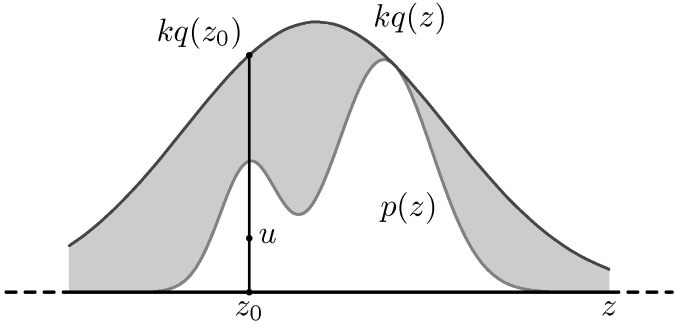
\includegraphics[scale=.5]{img/rejectionSampling.png}
\end{center}

\remarkk{Comments on Rejection Sampling}
\begin{itemize}
	\item[-] If the bound between $k.q(\cdot)$ \& $p(\cdot)$ is tight then the sample is efficient. Otherwise it can be wanting.
	\item[-] Often teh bound between $k.q(cdot)$ \& $p(\cdot)$ is not tight as we have to set $k$ very high.
	\item[-] Technique does not scale well to multiple dimensions.
	\item[-] Lots of samples get rejected.
\end{itemize}

\definition{Importance Sampling}
\textit{Importance Sampling} is a technique for approximating the \textit{Expected Value} of a distribution.\\
Suppose we wish to calcualte an expectation of $f(\cdot)$ wrt probability distribution $p(\cdot)$.\\
Chose a tractable distribution $q(\cdot)$ st $q(x)=0\implies p(x)=0$. Then we make the following approximation
$$\displaystyle{\expect[f(x)]\approx\frac{1}{N}\sum_{i=1}^Nf(x_i)\frac{p(x_i)}{q(x_i)}}$$
where $\{x_1,\dots,x_N\}$ is a sample from $q(x)$.\\

\prooff{Definition 5.7}
$$\displaystyle{\expect[f(x)]:=\int_\mathcal{X} f(x)p(x)dx=\int_\mathcal{X} f(x)\frac{q(x)}{q(x)}p(x)dx=\int_\mathcal{X} f(x)\frac{p(x)}{q(x)}q(x)dx=\expect_{q(\cdot)}\left[f(x)\frac{p(x)}{q(x)}\right]\approx\frac{1}{N}\sum_{i=1}^Nf(x_i)\frac{p(x_i)}{q(x_i)}}$$

\remarkk{Comments on Importance Sampling}
\begin{itemize}
	\item[-] Accepts all samples.
	\item[-] $\dfrac{p(\cdot)}{q(\cdot)}$ is called the \textit{Sampling Ratio} and acts to correct the bias caused by sample from the wrong distribution.
	\item[-] We cannot have $q(x_i)=0$ for any $i\in[1,N]$.
	\item[-] We may not always be to evaluate $p(\cdot)$.
\end{itemize}

\definition{Markov Chain Monte Carlo}
\textit{Markov Chain Monte Carlo}, MCMC, methods are techniques for generating observations from a distribution and they work well with multi-dimensional continous random variables.\\
Let $p(\cdot)$ be the distribution we wish to sample from, $\x_t$ be a state at time $t$ and $q(\cdot)$ be a proposed distribution which we can sample from.
\begin{enumerate}
	\item Initalise a state, $\x_0$. Set $t=0$.
	\item While time limit has not been reached
	\begin{enumerate}[label=\arabic*)]
		\item Sample a point, $\x'$, from the proposed distribution, $q(\cdot)$.
		\item Compute an acceptance probability
		$$A(\x',\x_t):=\min\left\{1,\frac{p(\x')}{p(\x_t)}\right\}$$
		\item Sample a point, $u$, from $\text{Uniform}[0,1]$.
		\begin{enumerate}
			\item If $A(\x',\x_0)>u$ then set $\x_{t+1}=\x'$.
			\item Otherwise, set $\x_{t+1}=\x_t$.
		\end{enumerate}	
		\item Increment $t$
	\end{enumerate}
\end{enumerate}
This can be visualised as a chain which works its way through the domain space, but backtracks every time it does not make a sample.
\begin{center}
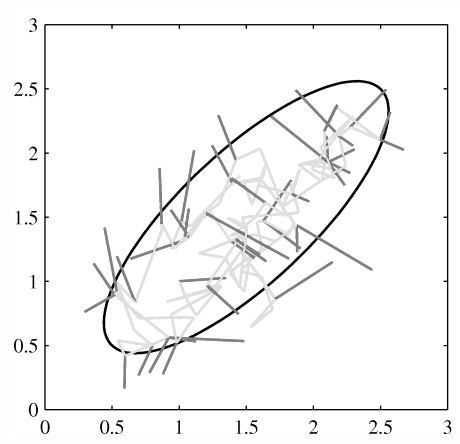
\includegraphics[scale=.5]{img/mcmc.png}
\end{center}

\remarkk{Commnets on Markov Chain Monte Carlo}
\begin{itemize}
	\item[-] Has the \textit{Markov Property}. (\ie Remembers its state from the last sample \& uses it).
	\item[-] Good at exploring.
\end{itemize}

\definition{Gibbs Sampling}
\textit{Gibbs Sampling} is an application of the \textit{Markov Chain Monte Carlo} algorithn. \textit{Gibbs Sampling} exploits the fact that $1$-Dimensional samples are often easier to generate by only every sampling from a single dimension.
Let $p(\cdot)$ be the distribution we wish to sample from, $\x_t$ be a state at time $t$ and $q(\cdot)$ be a proposed distribution which we can sample from.
\begin{enumerate}
	\item Initalise a state $\x_0$. Set $t=0$.
	\item While time limit has not been reached.
	\begin{enumerate}
		\item For each dimension $i$:
		\begin{enumerate}[label=\arabic*)]
			\item Isolate the dimension, $x_{t,i}$, from $\x_t$.
			\item Define $\x_{t,\neg i}:=\x_t/x_{t,i}$ to be $\x_t$ without its $i^\text{th}$ dimension.
			\item Calculate the \textit{posterior} for this dimension, conditional on $\x_{t,\neg i}$.
			$$p(x_{t,i}|\x_{t,\neg i})$$
			\item Sample a point, $x_{t+1,i}$, from $p(x_{t,i}|\x_{t,\neg i})$.	
		\end{enumerate}
		\item Increment $t$
	\end{enumerate}
\end{enumerate}

\subsection{Deterministic Techniques}

\definition{Deterministic Techniques for Approximative Inference}
\textit{Deterministic Techniques} for \textit{Approximative Inference} rely on making analytical approximations about the \textit{posterior} distribution in order to make it tractable.\\
Often these assumptions are about the particular distribution the \textit{posterior} takes or how it factorises.\\

\definition{Variational Bayes}
\textit{Variational Bayesian Methods} are techniques used for approximating intractable distributions which arise in \textit{Bayesian Inference}.\\
Let $\{X,Y\}$ be a set of training data. From \textit{Bayes' Theorem} we have that the \textit{evidence} is
$$p(Y)=\frac{p(Y|X)p(X)}{p(X|Y)}$$
Both $p(Y|X)$ and $p(X)$ are known, thus only $p(X|Y)$ is intractable.\\
Thus in order to approximate the \textit{evidence}, $p(Y)$, we need to approximate the \textit{posterior}, $p(X|Y)$.\\

\theoremm{Jensen's Inequality}
The function of the expected value is a lower bound to the expected value of the function.
\[\begin{array}{rcl}
\expect[f(X)]&\geq&f(\expect(X))\\
\displaystyle\int f(x)p(x)dx&\geq&f\left(\displaystyle\int xp(x)dx\right)
\end{array}\]
\nb Often we use this for $f(x)=\ln x$ as logs make many problems easier.\\

\definition{Kullback-Leibler Divergence}
\textit{Kullback-Leibler Divergence} measures the divergence between two distributions.\\
It is not symmetric \& thus is not a metric.\\
Let $p(X)$ and $q(X)$ be probability distributions we wish to compare. Then
$$KL(q(X)||p(X)):=\int q(X)\ln\dfrac{q(X)}{p(X)}dX$$
\nb The \textit{KL} measure requires that $q(X)$ \& $p(X)$ be zero-matching. \ie Whenever one of them equals 0 the other must too. This causes some limitations.\\

\remarkk{Features of Kullback-Leibler Divergence}
\begin{enumerate}
	\item $KL(q(x)||p(x))=0\Longleftrightarrow q(x)=p(x)$.
	\item $KL(q(x)||p(x))\geq0$.
\end{enumerate}

\proposition{Variational Bayes}
Here we shall reformulate the inference problem as an \textit{optimisation} problem.\\
Let $p(\textbf{Y})$ be an intractable distribution we are trying to approximate \& choose $q(\X)$ to be a tractable distribution.\\
The idea is to choose $q(\X)$ st it is approximately equal to $p(\X)$.
\[\begin{array}{rcl}
\ln p(\textbf{Y})&=&\ln\left(\displaystyle\int p(\textbf{Y},\X)d\X\right)\text{ by definition of evidence}\\
&\vdots&\\
&\geq&\displaystyle\int q(\X)\ln\left(\dfrac{p(\X|\textbf{Y})p(\textbf{Y})}{q(\X)}\right)d\X\text{ by Jensen's Inequality}\\
&\vdots&\\
&=&-KL(q(\X)||p(\X|\textbf{Y}))+\ln p(\textbf{Y})
\end{array}\]
Consider the \textit{Kullback-Leibler Divergence} element of this derivation as this is the term we are seeking to minimise (\ie make as close to zero as possible).
\[\begin{array}{rrl}
KL(q(\X)||p(\X|\textbf{Y}))&:=&\displaystyle\int q(\X)\ln\left(\dfrac{q(\X)}{p(\X|\textbf{Y})}\right)d\X\\
&\vdots&\\
&=&H(q(\X))-\expect_{q(\x)}[\ln p(\X,\textbf{Y})]+\ln p(\textbf{Y})\\
\implies\ln p(\textbf{Y})&=&KL(q(\X)||p(\X,\textbf{Y}))+\expect_{q(\X)}[\ln p(\X,\textbf{Y})-H(q(\X))\\
&\geq&\expect_{q(\X)}[\ln p(\X,\textbf{Y})]-H(q(\X))\text{ since }KL(\cdot||\cdot)\geq0\\
\text{Define }L(q(\X))&:=&\expect_{q(\X)}[\ln p(\X,\textbf{Y})]-H(q(\X))\text{ called Evidence Lower BOund (ELBO)}
\end{array}\]
We have now derived a likelihood function, $L(q(\X))$, for our proposed approximate distribution which we seek to maximise.\\
Note the following are valid expressions of our likelihood function
$$L(q(\X)):=\expect_{q(\x)}[\ln p(\X,\textbf{Y})]-H(q(\X))=\int q(\X)\ln\dfrac{p(\textbf{Y},\X)}{q(\X)}d\X\text{ by log rules}$$
\nb Maximising $L(q(\X))$ is equivalent to minimising $KL(q(\X)||p(\X,\textbf{Y}))$ which in turns implies $q(\X)$ and $p(\X,\textbf{Y})$ are very similar, as desired.\\

\proposition{Using result of Variational Bayes}
Remembering that $q(\X)$ is an approximation of the true posterior $p(\X|\textbf{Y})$.\\
Using the likelihood function, $L(\cdot)$, derived in \textbf{Proposition 5.3} we want to find $q(\X)$ which maximises its value since all other terms are known.\\
Note that if we can \underline{not} formulate the joint distribution, $p(\X,\textbf{Y})$, we are no better off using this derivation.

\subsubsection{Mean Field Approximation}

\remark{Motivation}
Now we have managed to redefine the inference problem as an optimisation problem we need to consider possible distributions for $q(\X)$ which we can then test. \textit{Mean Field Approximation} is a specific family of approximations, $q(\X)$, where we assume that each data point is independent and update the distribution of each point over a series of cycles.
$$q(\X):=\prod_iq_i(X_i)$$

\proposition{Mean Field Approximation}
Consider the likelihood function for \textit{variational inference} derived in \textbf{Proposition 13.2} and the definition of $q(\X)$ we are using
\[\begin{array}{rcl}
L(q(\X))&=&\displaystyle\int q(\X)\ln\dfrac{p(\textbf{Y},\X)}{q(\X)}d\X\\
&=&{\displaystyle\int\prod_iq_i(X_i)\ln\dfrac{p(\textbf{Y},\X)}{\prod_kq_k(X_k)}d\X}\\
&=&{\displaystyle\int\prod_iq_i(X_i)\left(\ln p(\textbf{Y},\X)-\sum_k\ln q_k(X_k)\right)d\X}
\end{array}\]
Since we want to update the distribution of each data point we note that our likelihood function can be rewritten as
$$L(q)=L(q_j)+L(q_{\neg j})$$
where $j$ is a data point we are interested in at this point in time.\\
Thus we can derive the likelihood function for proposed distributions of this form
\[\begin{array}{rcl}
L(q)&=&{\displaystyle\int\prod_iq_i(X_i)\left(\ln p(\textbf{Y},\X)-\sum_k\ln q_k(X_k)\right)d\X}\\
&\vdots\\
&=&-KL(q_j(X_j)||f_j(X_j))+c
\end{array}\]
Again our task is to minimise $KL(\cdot||\cdot)$. We know that $KL(\cdot||\cdot)\geq0$ the minimal value for $KL$ is 0 (the case where $q_j=f_j$).\\
Since we are free to choose $q_j(X_j)$ we can simply equate it with $f_j(X_j)$.\\
Consider the defintion of $f_j(X_j)$ from the previous derivation
$$\ln f_j(X_j):=\int_{\neg j}\prod_{i\neq j}q_i(X_i)\ln p(\textbf{Y},\X)d\X_{\neg j}=\expect_{q_{\neg j}(X_{\neq j})}[\ln p(\textbf{Y},\X)]$$
Thus we need to choose a distribution, $q_j(X_j)$, where the above expectation is tractable.\\

\proposition{Mean Field Approximation - Ising Model}
THIS IS A VERY LONG DERIVATION WHICH IS IN FULL NOTES.\\
LOOK AT LATER.

\section{Reinforcement Learning}

\definition{Reinforcement Learning}
\textit{Reinforcement Learning} aims to learn a solution to a task without specifying the task explicitly. Instead we define a system which rewards the computer for doing good actions.\\
We wish to learn a \textit{policy}, $\pi$, which decides what action will produce the greatest reward in any given state.\\
We note that the model is not stationary as it should evolve over time, as it recieves rewards (in effect learning). This means we have to collect new data each iteration.\\

\propositionn{Reinforcement Learning Process}
\begin{enumerate}[label=\arabic*)]
	\item Until time limit is reached
	\begin{enumerate}[label=\roman*)]
		\item Agent takes the action it believes will give the greatest reward.
		\item The environment changes accordingly.
		\item The agent recieves some reward (dependent upon how good the action was).
	\end{enumerate}
	\item Backpropogate results (learning).
\end{enumerate}

\proposition{Assessing Optimal Behaviour}
Depending on the task we may wish to adjust how we measure \textit{Optimal Behaviour} wrt time
\begin{enumerate}
	\item \textit{Finite Time Horizon} - Sum of scores up to a specific time point.
	$$\expect\left(\sum_{t=0}^Tr_t\right)$$
	\item \textit{Infnite Time Horizon} - Sum of scores over all time, with decaying relevance.
	$$\expect\left(\sum_{t=0}^\infty\gamma^tr_t\right)\text{ for }\gamma\in[0,1]$$
	\item \textit{Average Reward over Infinite Time} - Average score per time period.
	$$\lim_{T\to\infty}\expect\left(\frac1T\sum_{t=0}^Hr_t\right)$$
\end{enumerate}

\newpage
\setcounter{section}{-1}
\section{Reference}

\remark{Useful Links}
\textit{https://katbailey.github.io/post/gaussian-processes-for-dummies/}\\
\textit{https://www.quora.com/What-is-the-difference-between-backpropagation-and-gradient-descent-when-training}\\\textit{-a-deep-learning-neural-network-Which-of-the-two-is-Tensorflow-using}\\
\textit{https://www.youtube.com/watch?v=0NMC2NfJGqo}\\

\remark{Interpretting a data set}
Let $\X$ be a matrix which represents a set of data.\\
Rows of $\X$ will represent a single observation and columns will reprensent all observations of a given variable.\\

\definition{Basis Functions}
\textit{Basis Functions} are sets of functions from which all functions in their space can be decomposed into a linear combination of them. \textit{Basis Functions} cannot themselves be decomposed any further.
\begin{center}\begin{tabular}{l|l}
Polynomial Basis&$\{f_i(x)=x^i:i\in\nats_0\}$\\
Fourier Bais&$\{f(x)=\sin(x),f(x)=\cos(x)\}$
\end{tabular}\end{center}

\theorem{Schur Complement}
Let $M\in\reals^{p\times q}$ be a general matrix with block decomposition $\begin{pmatrix}E&F\\G&H\end{pmatrix}$.\\
The \textit{Schur Complement} is a tool used for inverting matrices as it isolates the problem to only needing to know the inverse of block $H$.\\
$$M^{-1}=\begin{pmatrix}(E-FH^{-1}G)^{-1}&-(E-FH^{-1}G)FH^{-1}\\-H^{-1}G(E-FH^{-1}G)^{-1}&H^{-1}+H^{-1}G(E-FH^{-1}G)FH^{-1}\end{pmatrix}$$
Here $E-FH^{-1}G$ is called the \textit{Schur Complement} of $M$ wrt $H$.\\
\nb This is denoted as $M/H$.\\

\definition{Exlpaining Away}
\textit{Explaining Away} is the process of breaking down a feature into multiple features in such a way that you isolate a particular variable of that feature. This is useful as we may not know much about the original feature, but a lot about the sub-features.\\

\definition{Hierarchical Knowledge}
\textit{Hierarchical Knowledge} is an application of \textit{Explaining Away} where we apply it to the sub-features in order to produce a series of linear sub-$\dots$-sub features until we reach features which we have sufficient knowledge about.


\definition{Kernel}
The \textit{Kernel} of a function is all the elements in teh input that maps to a defined point in the output space, $x'$.
$$\text{Kern}(f):=\{x':f(x')=x'\}$$
\nb Often $x':=0$.\\
Note that $\text{Kern}(f_1)\subseteq\text{Kern}(f_2\circ f_1)\subseteq\dots\subseteq\text{Kern}(f_N\circ\dots\circ f_1)$.\\

\definition{Image}
The \textit{Image} of a function is the set of all possible output values a function can produce
$$\text{Im}(f):=\{f(x):x\in X\}$$
where $f:X\to Y$.\\
Note that $\text{Im}(f_N\circ\dots\circ f_1)\subseteq\dots\subseteq\text{Im}(f_N\circ f_{N-1})\subseteq\text{Im}(f_N)$.\\

\definitionn{Sigmoid Function}
$$\sigma(z):=\frac{1}{1+e^{-z}}$$

\definition{Ising Model}
The \textit{Ising Model} is a simple example of an undirected graphical model (Markov Random Fields).\\
The \textit{Ising Model} has a prior of the form
$$p(\x)=\frac{1}{Z_0}e^{E_0(\x)}$$
where $Z_0$ is a normalising factor \& $E_0(\cdot)$ is a function that is learge if $\x$ is somethign we believe is likely, otherwise it is small.\\
In scenarios where $x_i\in\{-1,1\}\ \forall\ i$ a good definition for $E_0(\cdot)$ is
$$E_0(\x)=\sum_{i=1}^N\sum_{j\in\mathcal{N}_i}w_{ij}x_ix_j$$
where $\mathcal{N}_i$ is the neighbourhood of $x_i$ and $w_{ij}$ is the weight that $i$ gives the values of $x_j$, as it is only positive when $x_i=x_j$.\\

\definition{Gradient Descent}
\textit{Gradient Descent} is an \underline{iterative} \textit{optimisaiton algorithm} which aims to find the local minimum of a function, and thus the parameters which produce it.\\
\textit{Gradient Descent} can be used in scenarios where a function is intractable, which \textit{Least Squares} \underline{cannot}.
\begin{enumerate}
	\item Set $t=0$.
	\item Randomly initalise parameter values, $\theta_t$.
	\item Repeat until convergence of $\theta_t$.
	\begin{enumerate}
		\item Evaluate the performance of this state using a \textit{Loss Function}, $L(\x,\theta_t)$.
		\item Find the derivative of the \textit{Loss Function} wrt the parameters, $\frac{d}{d\theta}L(\x,\theta)$.
		\item Evaluate the derivative for the parmater values we just tested, $z$.
		\item Calculate \textit{Step Size} $s:=z\times\alpha$, where $\alpha$ is the \textit{Learning Rate} $(\approx 0.1)$.
		\item Set $\theta_{t+1}=\theta_t-s$.
	\end{enumerate}
\end{enumerate}
\nb \textit{Sum of the Squared Residuals} is a good loss function, $L(\x,\theta):=\sum_i[o_i-e_i]^2$ where $o_i$ is the observed value \& $e_i$ is the predict value at a given point.\\

\definition{Eigenvalues \& Eigenvectors}
\textit{Eigenvalues} \& \textit{Eigenvectors} are properties of square matrices. For a square matrix $A\in M(\reals)_n$, $\lambda\in\reals$ \& $\pmb{v}\in\reals^n$ is an \textit{Eigenvalue} \& \textit{Eigenvector} pair of $A$ if
$$A\pmb{v}=\lambda\pmb{v}$$
\nb Solving $|A-\lambda I|=0$ produces in the eigenvalues of $A$, from which the eigenvectors can be found.\\

\subsection{Graphical Models}

\definition{Graphical Models}
\textit{Graphical Models} are graphs which shows the minimal factorisation for the joint distribution of all variables in a model. \textit{Graphical Models} are made up of a few core elements
\begin{itemize}
	\item[-] \textit{Nodes} - Variables (Random \& realisations).\\
	\nb We typically draw circles around random variables, with observed data being shaded, but not around constants.
	\item[-] \textit{Edges} - A stochastic relationship between varaibles.
	\item[-] \textit{Plates} (\ie groups of Nodes) - A product(\ie repeated variables).\\
	\ie Suppose we have independent random variables $\{X_1,\dots,X_N\}$ which all have the same dependencies, we can simplfy the graphical model by simply defining a generic random variable $X_i$ with the dependencies \& drawing a plate around $X_i$ which denotes the number of occurences.\\
	This can easily be extended for multiple variables with dependence.
\end{itemize}
The \textit{Edges} can be \textit{directed}, known as \textit{Bayesian Networks}, or \textit{\underline{un}directed}, known as \textit{Markoc Random Fields}.\\

\example{Plate Notation}
Below are examples of \textit{Graphical Models}, using Plate Notation, for common machine learning model
\begin{center}\begin{tabular}{cc}
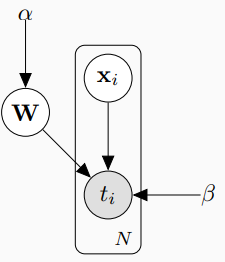
\includegraphics[scale=.5]{img/graphicalModel3.png}&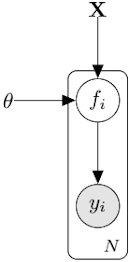
\includegraphics[scale=.5]{img/graphicalModel4.png}\\
Linear Regression&Gaussian Process Regression
\end{tabular}\end{center}

\remark{Interpretting Factorisation from Bayesian Network}
Let $A$ be a random variable \& $X_1,\dots,X_N$ be the parents of $A$.\\
Then we have the following factorisation of the joint distribution
$$p(A,X_1,\dots,X_N)=p(A|X_1,\dots,X_N)p(X_1)\dots p(X_N)$$
Note that $A$ may have other ancestors but we only consider its direct parents as all other dependencies will be encoded in the distribution of $A$'s parents.\\

\examplee{Interpretting Factorisation from Bayesian Network}
\begin{center}
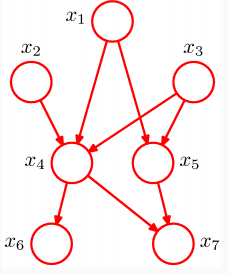
\includegraphics[scale=.5]{img/graphicalModel2.png}
\end{center}
$$p(x_1,\dots,x_7)=p(x_1)p(x_2)p(x_3)p(x_4|x_1,x_2,x_3)p(x_5|x_1,x_3)p(x_6|x_4)p(x_7|x_4,x_5)$$

\end{document}
